\chapter{Mathematical Model}

\section{Single Victim Case}
\begin{figure}[H]
    \centering
    \tdplotsetmaincoords{70}{110}
    \begin{tikzpicture}[tdplot_main_coords]
    \draw[thick,->] (0,0,0) -- (1,0,0) node[anchor=north east]{$y_g$};
    \draw[thick,->] (0,0,0) -- (0,1,0) node[anchor=north west]{$z_g$};
    \draw[thick,->] (0,0,0) -- (0,0,1) node[anchor=south]{$x_g$};
    % Point Pt1
    \coordinate (Pt1) at (5,0,5);
    \draw[->, thick] (0,0,0) -- (Pt1) node[pos=0.5,anchor=east]{${}^g \mathbf{p}_t$};      
    % Point tp
    \coordinate (p1) at (5,5,6);
    \draw[->, thick] (5,0,5) -- (p1) node[pos=0.5,anchor=south]{${}^t \bm{p}_{tr}$};      
    % pr
    \draw[->, thick] (0,0,0) -- (p1) node[pos=0.5,anchor=east]{${}^g \mathbf{p}_r$};

    \node at (p1) [anchor= south west] {$\mathbf{p}$};
    
    \coordinate (Shift) at (5,0,5);
    \tdplotsetrotatedcoordsorigin{(Shift)}
    \draw[thick,tdplot_rotated_coords,->] (0,0,0) --
    (.7,0,0) node[anchor=north]{$y_{t}$};
    \draw[thick,tdplot_rotated_coords,->] (0,0,0) --
    (0,.7,0) node[anchor=north]{$z_{t}$};
    \draw[thick,tdplot_rotated_coords,->] (0,0,0) --
    (0,0,.7) node[anchor=south]{$x_{t}$};
    \coordinate (Shift) at (5,5,6);
    \tdplotsetrotatedcoordsorigin{(Shift)}
    \draw[thick,tdplot_rotated_coords,->] (0,0,0) --
    (.7,0,0) node[anchor=east]{$y_{r}$};
    \draw[thick,tdplot_rotated_coords,->] (0,0,0) --
    (0,.7,0) node[anchor=west]{$z_{r}$};
    \draw[thick,tdplot_rotated_coords,->] (0,0,0) --
    (0,0,.7) node[anchor=south]{$x_{r}$};
    \end{tikzpicture}
    \caption{Inertial frames in the single victim case}
    \label{fig:frames-1victim}
\end{figure}
Three Cartesian coordinate frames are defined as \cite{main} and shown in \ref{fig:frames-1victim}:
\begin{enumerate}[label=(\roman*)]
    \item Frame $g$ (global): denoted as $F_g = (O_g, x_g, y_g, z_g)$, is the global (inertial) frame with origin $O_g$,
    fixed reference for all objects in space.
    \item Frame $r$ (receiver ARTVA): denoted as $F_r = (O_r, x_r, y_r, z_r)$, is the body right-hand frame associated with the receiver installed on the drone.
    \item Frame $t$ (transmitter ARTVA): denoted as $F_t = (O_t, x_t, y_t, z_t)$, is the body right-hand frame associated with the transmitter worn by the victim.
\end{enumerate}
For the sake of simplicity, we assume that the body frame of the drone coincides with $F_r$. 
The position of $O_r$ relative to $O_t$ is indicated by the vector $\mathbf{p}_{tr} \in \mathbb{R}^3$, with $\mathbf{p}_{tr} = \mathbf{p}_r - \mathbf{p}_t$, 
while the positions of $O_r$ and $O_t$ relative to $O_g$ are indicated, respectively, by the vectors $\mathbf{p}_r \in \mathbb{R}^3$ and $\mathbf{p}_t \in \mathbb{R}^3$.
We use the apex $g$, $r$ or $t$ on the left of the vector to indicate in which frame the vector is expressed , e.g. ${}^t p$. 
If it is not specified, we assume the global (inertial) frame.
We denote the \textit{special orthogonal group} of order three as \( \textit{SO}(3) \), 
which is the set of all \( 3 \times 3 \) orthogonal matrices with determinant equal to one:
\[
\textit{SO}(3) = \{ \mathbf{R} \in \mathbb{R}^{3 \times 3} \mid \mathbf{R}^\top \mathbf{R} = \mathbf{I}, \, \det(\mathbf{R}) = 1 \}
\]
Therefore, we indicate with \( \mathbf{R}_t^g \in \textit{SO}(3) \) a rotation matrix that rotates 
frame \( t \) into frame \( g \).

\noindent
As mentioned in the Introduction \ref{intro}, the ARTVA instrument can be equipped with three antennas aligned along 
the receiver frame axes \( x_r \), \( y_r \), and \( z_r \), corresponding to the longitudinal, 
lateral, and vertical directions of the sensor case, respectively. 
In both the single victim and multiple victims cases, we assume 
that the ARTVA receiver position \( \mathbf{p}_r \) and orientation \( \mathbf{R}_r \) in 
the inertial frame are known, as in \cite{main}. 

The electromagnetic field measured by the receiver, defined as  \( {}^r \mathbf{H} \), 
is given by the projection of vector field \( {}^t\mathbf{H} \) onto the \( F_r \) frame, 
corrupted by some sensor noise:
\begin{equation}
    {}^r\mathbf{H} =  \mathbf{R}^t_r \, {}^t\mathbf{H} + {}^r\mathbf{W}(t)
    \label{eq:H_rotated_noise}
\end{equation}
where \( {}^r\mathbf{W}(t) : \mathbb{R} \rightarrow \mathbb{R}^3 \) represents the 
EMI\footnote{EMI stands for electromagnetic interference} 
expressed in the receiver frame. 
Note that the noise is bounded and it is modeled as white noise 
${}^r\mathbf{W}(t) \sim \mathcal{N}(0, \sigma^2 \mathbf{I})$.

\subsection{Magnitude of Magnetic Field Intensity H}
We have found an expression of $\mathbf{H}$ in spherical coordinates, \ref{eq:H_spheric}, whose magnitude is found as:
\begin{equation}
    \left| \mathbf{H} \right| = \frac{I b^2}{4 \, r^3} \sqrt{ 4 \cos^2 \theta + \sin^2 \theta} = \frac{I b^2}{4 \, r^3} \sqrt{ 3 \cos^2 \theta + 1}
    \label{eq:H_mag_spher}
\end{equation}

\subsubsection{Approximation}
We use the same approximation in \cite{main} in order to remove the non-linearity given by the square root term $\sqrt{ 3 \cos^2 \theta + 1}$. Therefore we approximate:
\[
\frac{1}{\sqrt[3]{ 3 \cos^2 \theta + 1}} \approx \frac{1}{a^2 }\cos^2 \theta + \frac{1}{b^2} \sin^2 \theta
\]
of which the polar plot is shown in Figure \ref{fig:polarplot} when $a$ and $b$ have values 1.291 and 1.028, 
respectively, which minimize the relative mean squared error = 0.123\%.

% with the relative error this are instead the best values
% Best a: 1.284
% Best b: 1.034

Thus, the square root term becomes:
\begin{equation}
    \sqrt{ 3 \cos^2 \theta + 1} \approx \frac{1}{\left(\frac{1}{a^2} \cos^2 \theta + \frac{1}{b^2} \sin^2 \theta\right)^{3/2}}
    \label{eq:approx}
\end{equation}

Using the approximation \eqref{eq:approx} in \eqref{eq:H_mag_spher}:
\begin{equation}
    \left| \mathbf{H} \right| = \frac{I b^2}{4 \, r^3} \left(\frac{1}{a^2} \cos^2 \theta + \frac{1}{b^2} \sin^2 \theta\right)^{2/3}
    \label{eq:H_mag_approx}
\end{equation}

\begin{figure}[h!]
\centering
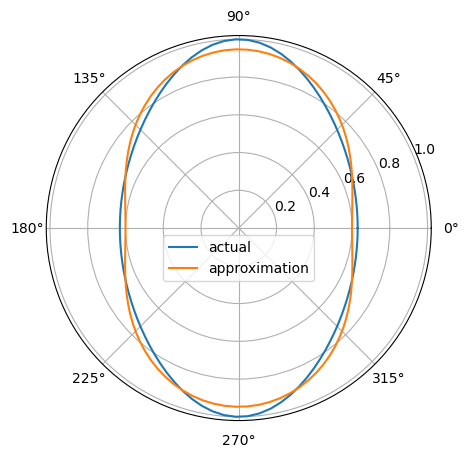
\includegraphics[width=0.5\textwidth]{images/polar_plot.png}
\caption{Polar plot of the actual function $\sqrt{ 3 \cos^2 \theta + 1} $ in blue 
and the approximated one $\frac{1}{a^2 }\cos^2 \theta + \frac{1}{b^2} \sin^2 \theta$ in orange.}
\label{fig:polarplot}
\end{figure}

Now we can express the magnitude using the Cartesian coordinates relative to the frame of the transmitter ARTVA $F_t$. 
If we consider the point ${}^t \mathbf{p}_{tr}$\[
    {}^t \mathbf{p}_{tr} = \begin{pmatrix}
    x \\
    y \\
    z
\end{pmatrix}
\] having these coordinates $(x,y,z)$ in frame $t$, then remembering $r$ from \ref{Conversion from Cartesian to Spherical Coordinates} and $\cos\theta$ from \ref{Conversion from Spherical to Cartesian Coordinates}:
\[
\begin{cases}
r^2 = x^2 + y^2 + z^2 \\
\cos\theta = \frac{x}{r}
\end{cases}
\]

Substituting the expressions for \(r\) and \(\cos\theta\) in \ref{eq:H_mag_approx}:
\[
\left| \mathbf{H} \right| = \frac{I b^2}{4} \frac{1}{(x^2 + y^2 + z^2)^{3}} \left(\frac{1}{a^2} \frac{x^2}{x^2 + y^2 + z^2} + \frac{1}{b^2} \frac{y^2 + z^2}{x^2 + y^2 + z^2}\right)^{2/3}
\]

After simplifications and further calculations, we obtain:
\begin{equation}
    \left| \mathbf{H} \right| = \frac{m}{4 \pi} \left(\frac{(ab)^2}{b^2 x^2 + a^2 (y^2 + z^2)}\right)^{3/2}
    \label{eq:H_mag_cart}
\end{equation}
where we call $I \, \pi \, b^2$ the magnetic moment $m$, as seen in \ref{eq:magnetic_moment}.
Then, we can define $\eta$ as \cite{main}:
\[ \eta = \left( \frac{m}{4 \pi \left| \mathbf{H} \right|} \right)^{2/3} \cdot \, (ab)^2 = \]
by substituting \ref{eq:H_mag_cart}:
\[
\begin{aligned}
&= \left( \frac{m}{4 \pi \frac{m}{4 \pi} \left(\frac{(ab)^2}{b^2 x^2 + a^2 (y^2 + z^2)}\right)^{3/2}} \right)^{2/3} \cdot (ab)^2 = 
\\
&= \left( \left(\frac{b^2 x^2 + a^2 (y^2 + z^2)}{(ab)^2}\right)^{3/2}\right)^{2/3} \cdot (ab)^2
\end{aligned}
\]

So:
\begin{equation}
    \eta = b^2 x^2 + a^2 (y^2 + z^2)
    \label{eq:eta}
\end{equation}

\subsection{Finding the ARTVA position}
In order to find the victim's position $\mathbf{p}_t$ with respect to the global frame $F_g$, we need to use homogeneous transformations \cite{book-robotics}. 
Also from Figure \ref{fig:frames-1victim}, we can express the position of the receiver $\mathbf{p}_r$ in the inertial (global) frame as the sum of the other two vectors:
\[
\begin{aligned}
{}^g \mathbf{p}_r &= {}^g \mathbf{p}_t + {}^t \mathbf{p}_{tr} \\
{}^t \mathbf{p}_{tr} &= \mathbf{R}_t^g \,\, {}^g \mathbf{p}_{tr}
\end{aligned}
\]
where $\mathbf{R}_t^g$ is the rotation matrix that rotates frame $g$ to $t$ \cite{artva-gazebo}.
\begin{comment}
The matrix $R_t^i$ is the matrix which lets us express the vector in frame $i$ using the coordinates of the vector in frame $t$.Since we are expressing in the columns the coordinates of the axis of $t$ w.r.t using the axis of $i$.
Then if we have the coordinates of point $P$ with respect to frame i $\mathbf{P}$ 
(and if we know the rotation that goes from frame $i$ to frame $t$ (which also means we know the orientation and coordinates of the axis of frame $t$ with respect to those of frame $i$ $(R_t^i$ notation of Soper/this Chapman book), 
we can find the coordinates at point $P$ w.r.t frame i which is $\mathbf{P}$.
Also consider that from frame $i$ after a rotation $R_t^i$ we obtain the same orientation of frame $t$ which is just translated by the $\mathbf{P}_R$ vector.
v1 is  coordinates of the point before the translation but after the rotation, the coordinate of the point wrt the inertial frame  i are v1^i = R p^{i2}
\end{comment}

From which we can find $\mathbf{p}_t$ by multiplying by ${\mathbf{R}_t^g}^\top$ since ${\mathbf{R}_t^g}$ is orthogonal (${\mathbf{R}_t^g}^\top = {\mathbf{R}_t^g}^{-1}$):

\begin{equation}
    {}^t \mathbf{p}_{tr} = {\mathbf{R}_t^g}^\top (\mathbf{p}_r - \mathbf{p}_t)
    \label{eq:pt}
\end{equation}

In addition, remembering how we defined the coordinates of ${}^t \mathbf{p}_{tr}$, then from linear algebra:
\[
\begin{aligned}
x &= \mathbf{e}_x^\top \, {}^t \mathbf{p}_{tr} \\
y &= \mathbf{e}_y^\top \, {}^t \mathbf{p}_{tr} \\
x  &= \mathbf{e}_z^\top  \, {}^t \mathbf{p}_{tr}
\end{aligned}
\]
also,
\[
x^2 = x \cdot x = \left( \mathbf{e}_x^\top \, {}^t \mathbf{p}_{tr} \right)^\top \cdot \, \left( \mathbf{e}_x^\top \, {}^t \mathbf{p}_{tr} \right)
\]
and the same is valid for the other two coordinates, we will omit the calculations for the other two from now on. 
We can then substitute the expression we found for ${}^t \mathbf{p}_{tr}$ \ref{eq:pt} and apply linear algebra properties of the transpose:
$$(\mathbf{A}\mathbf{B}\mathbf{C})^\top = \mathbf{C}^\top \mathbf{B}^\top \mathbf{A}^\top$$ to calculate the transpose of $\mathbf{e}_x^\top {\mathbf{R}_t^g}^\top (\mathbf{p}_r - \mathbf{p}_t)$:

\[
(\mathbf{e}_x^\top {\mathbf{R}_t^g}^\top (\mathbf{p}_r - \mathbf{p}_t))^\top = (\mathbf{p}_r - \mathbf{p}_t)^\top {\mathbf{R}_t^g} \mathbf{e}_x
\]
The expression for $x^2$ then becomes:
\begin{equation}
    x^2 = \left(\mathbf{p}_r - \mathbf{p}_t\right)^\top {\mathbf{R}_t^g} \mathbf{e}_x \mathbf{e}_x^\top {\mathbf{R}_t^g}^\top \left(\mathbf{p}_r - \mathbf{p}_t\right)
    \label{eq:x2}
\end{equation}

Furthermore:
\[
\mathbf{e}_x \mathbf{e}_x^\top =\begin{pmatrix}
1 \\
0 \\
0
\end{pmatrix}
\begin{pmatrix}
1 & 0 & 0
\end{pmatrix}
 = \text{diag}(1,0,0)
\]
and:
\[
\begin{aligned}
    \mathbf{e}_y \mathbf{e}_y^\top &= \text{diag}(0,1,0) \\
    \mathbf{e}_z \mathbf{e}_z^\top &= \text{diag}(0,0,1)
\end{aligned}
\]
Lastly we substitute the result found in \ref{eq:x2} in the expression of $\eta$ \ref{eq:eta}:
\[
\begin{aligned}
    \eta &=  \ b^2 \left(\mathbf{p}_r - \mathbf{p}_t\right)^\top \mathbf{R}_t^g \mathbf{e}_x \mathbf{e}_x^\top {\mathbf{R}_t^g}^\top \left(\mathbf{p}_r - \mathbf{p}_t\right) + \\
    &+ a^2 \left(\mathbf{p}_r - \mathbf{p}_t\right)^\top \mathbf{R}_t^g \mathbf{e}_y \mathbf{e}_y^\top {\mathbf{R}_t^g}^\top \left(\mathbf{p}_r - \mathbf{p}_t\right) +\\
    &+ a^2 \left(\mathbf{p}_r - \mathbf{p}_t\right)^\top \mathbf{R}_t^g \mathbf{e}_z \mathbf{e}_z^\top {\mathbf{R}_t^g}^\top \left(\mathbf{p}_r - \mathbf{p}_t\right) =
\end{aligned}
\]
collect common terms,
\[
= \left(\mathbf{p}_r - \mathbf{p}_t\right)^\top \mathbf{R}_t^g \left( b^2 \mathbf{e}_x \mathbf{e}_x^\top + a^2 \mathbf{e}_y \mathbf{e}_y^\top + a^2 \mathbf{e}_z \mathbf{e}_z^\top \right) {R_t^g}^\top \left(\mathbf{p}_r - \mathbf{p}_t\right)=
\]
\begin{equation}
    = \left(\mathbf{p}_r - \mathbf{p}_t\right)^\top \mathbf{R}_t^g \, \text{diag}(b^2, a^2, a^2) {\mathbf{R}_t^g}^\top \left(\mathbf{p}_r - \mathbf{p}_t\right)
    \label{eq:eta2}
\end{equation}

We call the \( \mathbf{R}_t^g \, \text{diag}(b^2, a^2, a^2) {\mathbf{R}_t^g}^\top \) matrix $\mathbf{M}$ and the diagonal matrix $\text{diag}(b^2, a^2, a^2)$ $D$.

\subsubsection{Symmetry of \( \mathbf{M} \)}
\textbf{Definition} \\
A matrix \( \mathbf{M} \in \mathbb{R}^{n \times n} \) is symmetric if and only if \( \mathbf{M} = \mathbf{M}^\top \).
\\
\textbf{Proof} \\
We compute \( \mathbf{M}^\top \):
\[
    \mathbf{M}^\top = \left( \mathbf{R}_t^g \mathbf{D} {\mathbf{R}_t^g}^\top \right)^\top = \left( {\mathbf{R}_t^g}^\top \right)^\top \mathbf{D}^\top {\mathbf{R}_t^g}^\top = \mathbf{R}_t^g \mathbf{D}^\top {\mathbf{R}_t^g}^\top
\]
Since \( \mathbf{D} \) is a diagonal matrix, it is equal to its transpose $\mathbf{D}^\top = \mathbf{D}$ :
$$
\mathbf{M}^\top =  \mathbf{R}_t^g D {\mathbf{R}_t^g}^\top = \mathbf{M}
$$

\subsubsection{Final expression for $\eta$}
By applying the distributive property to \ref{eq:eta2} and since M is symmetric:
\begin{equation}
    \eta = \mathbf{p}_r^\top \mathbf{M} \mathbf{p}_r - \mathbf{p}_r^\top \mathbf{M} \mathbf{p}_t - \mathbf{p}_t^\top \mathbf{M} \mathbf{p}_r+ \mathbf{p}_t^\top \mathbf{M} \mathbf{p}_t
    \label{eq:eta3}
\end{equation}
The vector $\mathbf{\hat{p}}_t$ gives an estimate of the true position $\mathbf{p}_t$ :
\[
\mathbf{\hat{p}}_t = \mathbf{M} \mathbf{p}_t
\]
and since $M$ is symmetric:
\[
\mathbf{\hat{p}}_t^\top =  \mathbf{p}_t^\top \mathbf{M}^\top = \mathbf{p}_t^\top \mathbf{M}
\]
We substitute these expressions in \ref{eq:eta3} and use the definition of the scalar product:
\[
\eta = \mathbf{p}_r^\top \mathbf{M} \mathbf{p}_r - \mathbf{p}_r^\top \mathbf{\hat{p}}_t - \mathbf{\hat{p}}_t^\top \mathbf{p}_r+ \mathbf{p}_t^\top \mathbf{M} \mathbf{p}_r = \mathbf{p}_r^\top \mathbf{M} \mathbf{p}_r - 2 \mathbf{p}_r^\top \mathbf{\hat{p}}_t + \mathbf{p}_t^\top \mathbf{M} \mathbf{p}_t
\]
If we define the coordinates of $\mathbf{p}_r$ :
\[
\mathbf{p}_r = \begin{pmatrix}
    x_r \\
    y_r \\
    z_r
\end{pmatrix}
\]
and
\[
    \mathbf{M} = \begin{pmatrix}
    m_{11} & m_{12} & m_{13} \\
    m_{12} & m_{22} & m_{23} \\
    m_{13} & m_{23} & m_{33} \\
\end{pmatrix}
\]
we can compute $\mathbf{p}_r^\top \mathbf{M} \mathbf{p}_r$:
\[
\mathbf{p}_r^\top \mathbf{M} \mathbf{p}_r = 
m_{11} \, x_r^2 \; + \; 2 \, m_{12} \, x_r \, y_r \; + \; 2 \, m_{13} \, z_r \, x_r \; + \;
m_{22} \, y_r^2 \; + \; 2 \, m_{23} \, y_r \, z_r \; + \; m_{33} \, z_r^2
\]
Then, we obtain a final expression for $\eta$ as in \cite{main}:
\begin{equation}
\begin{aligned}
\eta = & \ m_{11} \, x_r^2 + 2 \, m_{12} \, x_r \, y_r + 2 \, m_{13} \, z_r \, x_r \\
       & \ + m_{22} \, y_r^2 + 2 \, m_{23} \, y_r \, z_r + m_{33} \, z_r^2 \\
       & \ - 2 \, x_r \, x_t - 2 \, y_r \, y_t - 2 \, z_r \, z_t \\
       & \ + \mathbf{p}_t^\top \mathbf{M} \mathbf{p}_t
\end{aligned}
\label{eq:eta_final}
\end{equation}

\noindent
We can rewrite the expression of eta in vector form by defining a vector $\mathbf{\Phi}$,
which is a funcion of known variables:
\begin{equation}
\renewcommand{\arraystretch}{1}
\mathbf{\Phi}(\mathbf{p}_{r}) = 
\begin{pmatrix}
x_r^2 \\
2x_r y_r \\
2x_r z_r \\
y_r^2 \\
2y_r z_r \\
z_r^2 \\
-2x_r \\
-2y_r \\
-2z_r \\
1
\end{pmatrix}
\label{eq:Phi_vector}
\end{equation}
and a vector of unknown constants $\mathbf{x}$:
\begin{equation}
\renewcommand{\arraystretch}{1}
\mathbf{x}(\mathbf{p}_t) = 
\begin{pmatrix}
m_{11} \\
m_{12} \\
m_{13} \\
m_{22} \\
m_{23} \\
m_{33} \\
\mathbf{p}_t \\
\rho
\end{pmatrix}
\label{eq:x_vector}
\end{equation}  
where \( \rho := \mathbf{p}_t^\top \mathbf{M} \mathbf{p}_t \).

\noindent
Then $\eta$ exspressed in a compact vector form is:
\begin{equation}
    \eta = \mathbf{\Phi}^\top\mkern-2mu(\mathbf{p}_{r}) \, \mathbf{x}(\mathbf{p}_t)
    \label{eq:eta_final_final}
\end{equation}

\noindent
Afterward, we leverage the $\eta$ signal (function of the ARTVA output
of Eq. \ref{eq:H_rotated_noise}) to estimate the
the transmitter’s position \( \mathbf{p}_t \), which corresponds to the victim's location. 
We omit the estimation of the transmitter orientation \( \mathbf{R}^g_t \),
since it is not critical in either the single-victim or multiple-victim cases.

\subsubsection{Final Model}
\noindent
In the final model of the single-victim case, we consider one victim to 
which it is attached an ARTVA transmitter and \( m \in \mathbb{N} \) receivers, 
each rigidly attached to each drone. 
We define the position of the $k$-th drone at sample time \( \tau_i \) with \( \mathbf{p}_{r_k}(\tau_i) \in \mathbb{R}^3 \) 
where \( k, i \in \mathbb{N} \) and \( k = 1, \ldots, m \).

\noindent
As described in \cite{similar-main} and as seen in the previous sections, 
we model the intensity of the ARTVA signal using $\eta$ in Eq. \ref{eq:eta_final_final} 
as an output function of the form \( y : \mathbb{R}^3 \times \mathbb{R} \rightarrow \mathbb{R} \):
\[
y(\mathbf{p}_{r_k}, \tau_i) = \mathbf{\Phi}^\top\mkern-2mu(\mathbf{p}_{r_k}) \, \mathbf{x}(\mathbf{p}_t) + 
w_t(\mathbf{p}_{r_k}, \mathbf{p}_t, \tau_i),
\]
where $\mathbf{\Phi}(\mathbf{p}_{r_k})$ is the vector of known variables
relative to each $k$-th receiver and 
and \( w : \mathbb{R}^3 \times \mathbb{R} \rightarrow \mathbb{R} \) 
represents the measurement noise and model 
mismatch introduced by the approximation.
Note that $w$ is realted to the EMI defined in \ref{eq:H_rotated_noise}, as demonstrated in \cite{similar-main}.

\subsection{Recursive Least Square}
VA SPIEGATO MEGLIO COME SI FA RLS DECENTRALIZZATO? VA CITATO L RLS NON SONO RIUSCITO A TROVARLO
We propose a decentralized estimation algorithm to address our task of localizing avalanche 
victims. A decentralized approach offers several advantages over a centralized one, particularly 
in scenarios characterized by limited computational resources and large-scale deployments. 
By distributing computation across multiple agents (the UAVs), this method reduces computational 
overload, enhancing scalability as the number of agents increases.

Furthermore, decentralization provides improved robustness to "communication noise" by removing 
dependence on a central computation unit. This autonomy enables the system to adapt to varying 
communication conditions, such as intermittent information availability or delays, thus supporting 
continued operation in challenging environments such asmountain regions and adverse weather 
conditions, like in our scenario. While decentralized methods may exhibit slower convergence and slightly higher estimation 
errors due to partial information exchange, they remain effective and efficient in situations where 
centralized coordination is impractical or demands excessive resources.

\noindent
\\
To estimate the constant vector \( \mathbf{p}_t \), we assume the position of each 
UAV, \( \mathbf{p}_{r_k}(\tau_i) \), as known. 
Each UAV in the network collects data independently and transmits information only 
to its neighboring agents. Each UAV then employs its own instance of the estimation 
algorithm, populating the necessary matrices and vectors in the equations to 
generate an independent estimate of the victim’s position:
\[
\mathbf{Y}(\tau_i) = \mathbf{H}(\tau_i) \mathbf{x}(\mathbf{p}_t) + \mathbf{W}(\tau_i)
\]
where
\[
\mathbf{Y}(\tau_i) = \mathrm{col}(y(\mathbf{p}_{r_1}(\tau_i), \tau_i), \ldots, y(\mathbf{p}_{r_m}(\tau_i), \tau_i)),
\]
\[
\mathbf{H}(\tau_i) = \mathrm{col}(\mathbf{\Phi}^\top(\mathbf{p}_{r_1}(\tau_i)), \ldots, \mathbf{\Phi}^\top(\mathbf{p}_{r_m}(\tau_i))),
\]
\[
\mathbf{W}(\tau_i) = \mathrm{col}(w(\mathbf{p}_{r_1}(\tau_i),\mathbf{p}_t, \tau_i), \ldots, v(\mathbf{p}_{r_m}(\tau_i), \mathbf{p}_t, \tau_i)).
\]
The model above enables estimation of \( \mathbf{x} \) using the affine term 
\( \mathbf{H}(\tau_i) \) through the RLS \footnote{RLS stands for Recursive Least Squares} algorithm:
\[
\begin{cases}
    \hat{\mathbf{x}}(\tau_{i+1}) = \hat{\mathbf{x}}(\tau_i) + \mathbf{S}^{-1}(\tau_i)\mathbf{H}(\tau_i) \left( \mathbf{Y}(\tau_i) - \mathbf{H}(\tau_i)^\top \hat{\mathbf{x}}(\tau_i) \right) \\
    \mathbf{S}(\tau_{i+1}) = \beta \mathbf{S}(\tau_i) + \mathbf{H}(\tau_i)\mathbf{H}(\tau_i)^\top
\end{cases}
\]
where \( \beta \in (0, 1) \) is a forgetting factor, and \( \mathbf{S}(\tau_0) = \mathbf{S}_0 \in \mathbb{R}^{3 \times 3} \). 

\noindent
The transmitter's position is estimated by
\begin{equation}
    \hat{\mathbf{p}}_t(\tau_i) = \mathbf{x}^{-1}(\hat{\mathbf{x}}(\tau_i))
    \label{eq:mapping}
\end{equation}
where \( \mathbf{x}^{-1} : \mathbb{R}^{10} \rightarrow \mathbb{R}^3 \) is well-defined as shown in \cite{similar-main}. 

\noindent
Note that, in both the RLS method applied for the single-victim case and in the multiple-victim algorithm, 
we assume the use of a precise positioning system, such as an ideal GPS.

\subsection{Average Consensus Filter}

A PI-ACF\footnote{PI-ACF stands for Proportional Integral Average Consensus Filter} was employed to compute 
a decentralized moving average of the UAVs' estimates. 
The ACF dynamics equations are described below:
\[
\begin{cases}
    \dot{z}^k = \gamma(\alpha^k - z^k) - K_P \sum_{j \in \mathcal{N}_k} (z^k - z^j) + K_I \sum_{j \in \mathcal{N}_k} (\omega^k - \omega^j) \\
    \dot{\omega}^k = - K_I \sum_{j \in \mathcal{N}_k} (z^k - z^j)
\end{cases}
\]
where:
\begin{itemize}
    \item \( z^k \): moving average computed by the \( k \)-th UAV;
    \item \( \omega^k \): integral variable, representing cumulative error 
    with neighbors;
    \item \( \alpha^k \): time-varying set-point, mean of neighboring UAVs' estimates;
    \item \( \mathcal{N}_k \): set of neighbors of the \( k \)-th UAV;
    \item \( \gamma \): hyperparameter adjusting convergence rate;
    \item \( K_P \) and \( K_I \): proportional and integral control gains.
\end{itemize}
This consensus mechanism enables UAVs to converge to a shared moving average, 
as each minimizes differences with its neighbors. The tracking term \( \gamma(\alpha^k - z^k) \) 
guides the \( k \)-th UAV towards its set-point, while the proportional control term 
\( -K_P \sum_{j \in \mathcal{N}_k} (z^k - z^j) \) ensures alignment with its neighbors. 
The integral control term \( K_I \sum_{j \in \mathcal{N}_k} (\omega^k - \omega^j) \) 
adds cumulative adjustment based on historical differences, addressing steady-state errors.

This algorithm supports convergence of the UAVs to a common moving average, even with 
limited communication. It allows the fleet to track changing set-points while 
reducing differences with neighbors in order to reach consensus.

\subsection{Normalized Source Strength}
In both the single-victim and multiple-victims cases, we can find the the NSS not only numerically but also
analytically, in this section we will detail how we compute the NSS for a single source with both methods.

\subsubsection{Analitycal method}
Since we have an expression of the magnetic field intensity ${}^t \mathbf{H}$
in Cartesian coordinates (in the transmitter reference frame) \ref{eq:final_H}, we can compute the derivatives and therefore the
gradient tensor ${}^t \mathbf{G}$ analytically as:
\begin{equation}
{}^t \mathbf{G} = \frac{1}{r^{5/2}}
\scalebox{0.96}{$
\begin{bmatrix}
3 x (-2 x^2 + 3y^2 + 3z^2) & 3 y (-4 x^2 + y^2 + z^2) & 3 z (-4x^2 + y^2 + z^2) \\
3 y (-4 x^2 + y^2 + z^2) & 3 x (x^2 - 4 y^2 + z^2) & -15 x y z \\
3 z (-4 x^2 + y^2 + z^2) & -15 x y z & 3 x (x^2 + y^2 - 4 z^2)
\end{bmatrix}
$}
\label{eq:G_analit}
\end{equation}
where $r$ is of course the distance, $r = \sqrt{x^2 +y^2 +z^2}$.

Note once again the symmetry and traceless property of the gradient tensor 
$\mathbf{G}$ is evident, when we compute it explicitly.
Also note that for simplicity we computed the gradient using $\mathbf{H}$ and not $\mathbf{B}$,
since they vary only by the constant permeability $\mu$. 
We also omitted the constants $I$, $b$, since they don't depend on the coordinates $(x, y, z)$
neither, and therefore do not influence the results.

In Figure \ref{fig:gradients_single_anal}, we show the gradients for a single
source centered at the origin of the space, when the global frame 
$F_g$ coincides with the trasmitter (source) frame $F_t$ and also when there 
is no rotation between these frames and the receiver frame $F_r$ of the drones. 
In this way, we have that the magnetic field intensity ${}^t \mathbf{H} = {}^g \mathbf{H}$
can be computed using the inertial coordinates, and also the
NSS at any point in space coincides with the signal received by 
any drone located at that point.
The gradients are calculated on a grid of equally spaced points in the range $[-5, 5]$, when we fix the $z$ coordinates
at 3 m, considering a reasonable flying height for the drones.
We need to fix one coordinate in order to be able to plot 
a function of 3 variables, but also because we assume the drones
flying always at a fixed height, as it will be explained more in 
depth lately.   
\begin{figure}[h]
\centering
\hspace*{-0.2\textwidth} 
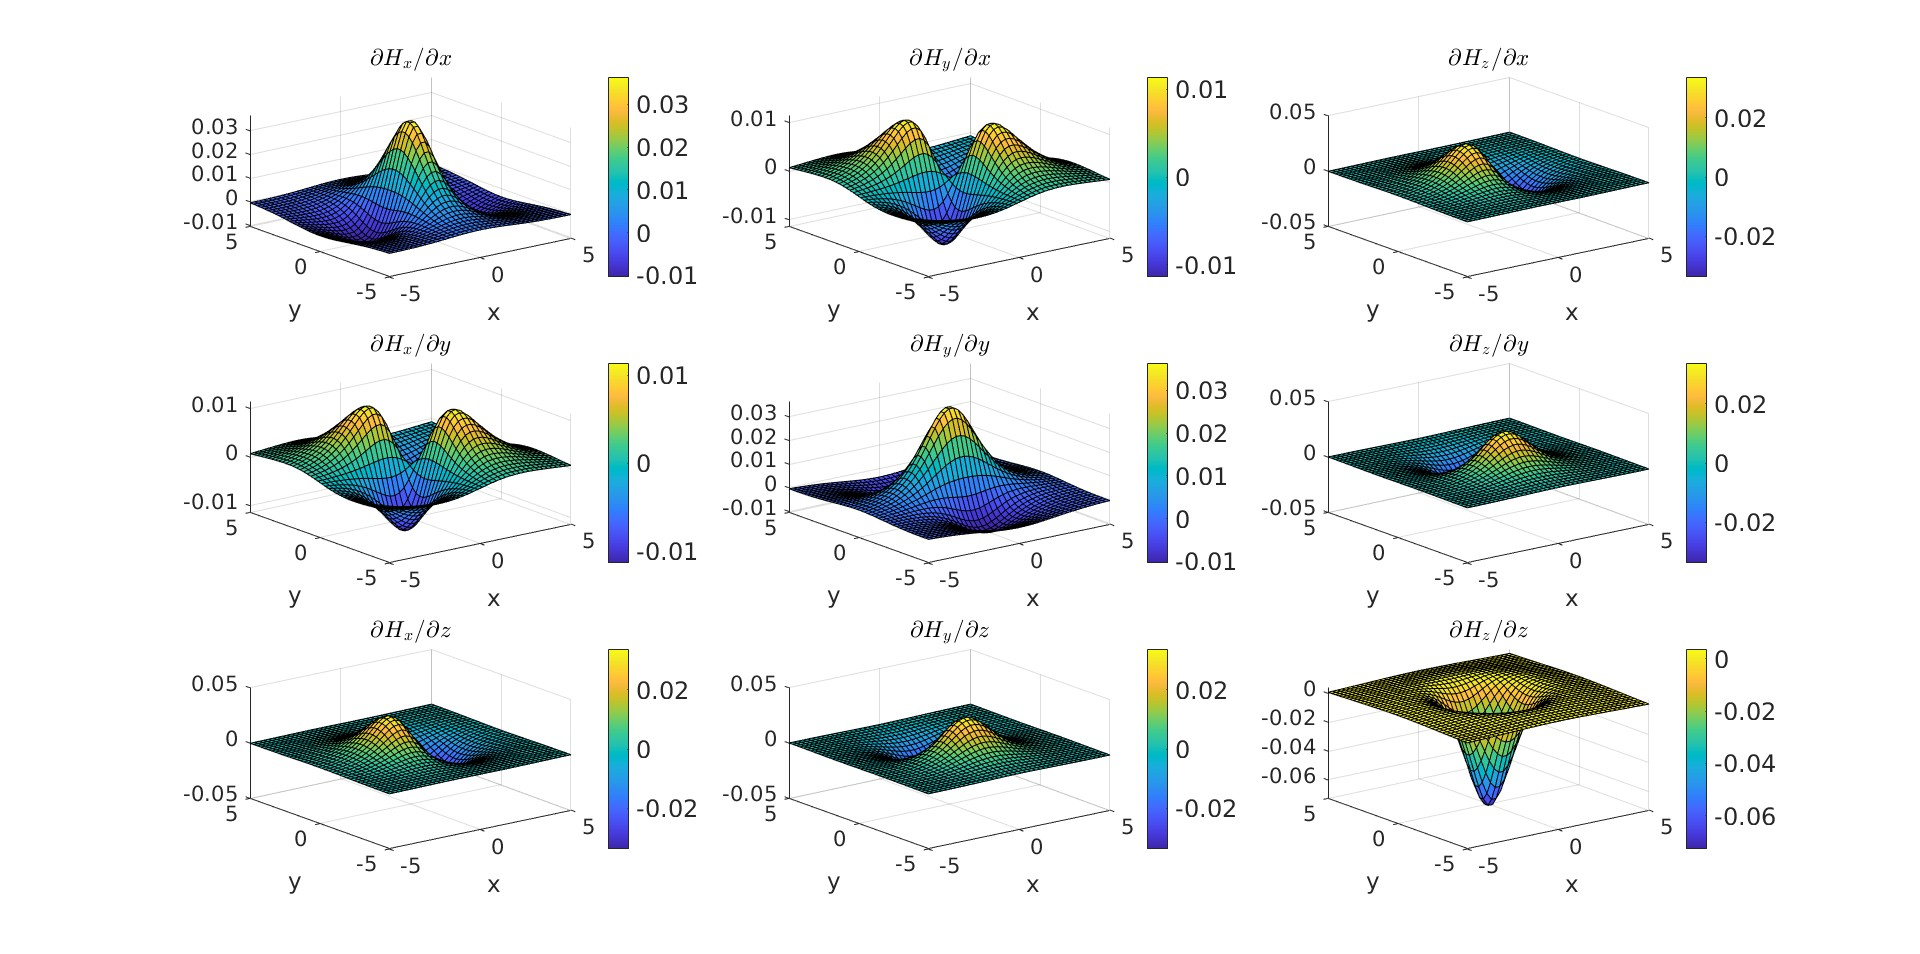
\includegraphics[width=1.4\textwidth]{images/gradients_single_anal.jpg}
\caption{Plot of the gradients \( \frac{\partial H_i}{\partial q_j} \), where \( i, j \in \{x, y, z\} \)
, $H_i$ are the scalar functions relative to the $i$-th component of the magnetic field 
intensity $\mathbf{H}$ and $q_j$ are the Cartesian coordinates.
The gradients are the components $H_{ij}$ of the gradient tensor \( \mathbf{G} \) when computed analytically as in Eq.~\ref{eq:G_analit}. 
This example considers a single source located at the center \((0,0,0)\) of the space, with no rotations 
between the coordinate frames \( F_g \), \( F_r \), and \( F_t \).}
\label{fig:gradients_single_anal}
\end{figure}

After having found the gradient tensor $\mathbf{G}$, we numerically
compute its eigenvalues and we find the NSS using the definition \ref{eq:NSS}.
In Figure \ref{fig:NSS_single_anal}, we plot the NSS distribution over the same grid,
with the same $z$ value fixed.
These values will be the signals received by the drones at their location
in space in the multiple victims case, which will be explained more in depth in the following paragraph.
\begin{figure}
\centering
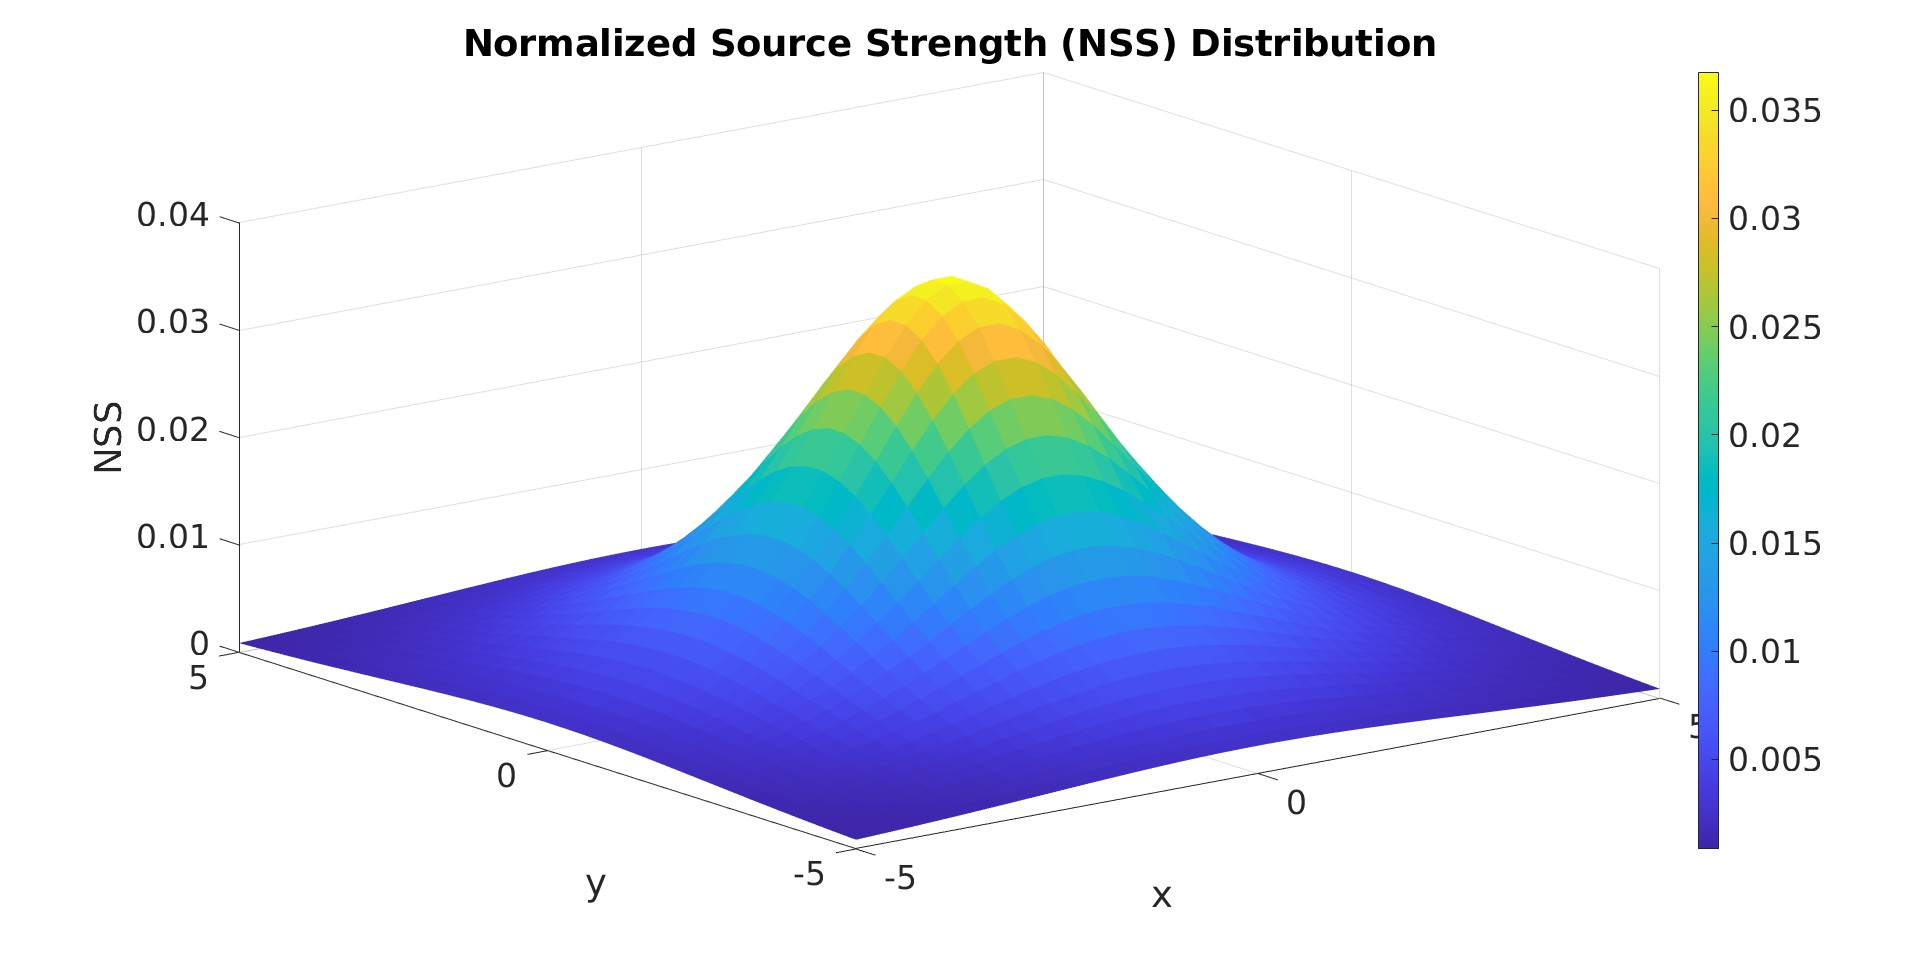
\includegraphics[width=0.8\textwidth]{images/NSS_single_anal.jpg}
\caption{Plot of the NSS values computed at each point on the grid, which
represent the signal received by the drones, in the case of a single source located
at the center $(0,0,0)$ of the space when there are no rotations between the coordinates
frames $F_g$, $F_r$, $F_t$..}
\label{fig:NSS_single_anal}
\end{figure}

Instead, let's consider the case when the source location is translated
with respect to the global frame $F_g$ and the transmitter frame $F_t$ is rotated
with respect to the same one by a rotation $\mathbf{R}_t^g$, like in the previous 
section.
Furthermore, we also consider the rotation $\mathbf{R}^t_r$ between the transmitter frame and the receiver
frame $F_r$.
Then, we compute the coordinates of any point in space with respect to the
transmitter frame as in \ref{eq:pt}.
Using these coordinates we find the magnetic intensity vector ${}^t\mathbf{H}$,
expressed in the trasmitter frame and compute the gradient tensor ${}^t \mathbf{G}$.
The magnetic field read by the receiver, denoted by ${}^r\mathbf{H}$, is given by the projection
of vector ${}^t\mathbf{H}$ onto the $F_r$ frame, as in Eq.\ref{eq:H_rotated_noise} but without considering
the noise for the moment:
\begin{equation}
    {}^r\mathbf{H} = \mathbf{R}^t_r \, {}^t\mathbf{H}
    \label{eq:H_receiver}
\end{equation}
Therefore, we apply Eq. \ref{eq:rotated_gradient_tensor} to find the gradient tensor
in the receiver frame, which represents the signal obtained in a real world scenario:
\begin{equation}
    {}^r \mathbf{G} = \mathbf{R}^t_r \, {}^t\mathbf{G} \, {\mathbf{R}^t_r}^\top
    \label{eq:G_rotated}
\end{equation}
In Figure \ref{fig:gradients_rotated_single_anal}, we see how the gradients plots
vary with respect to the gradients in Figure \ref{fig:gradients_single_anal},
since the rotations introduce naturally a modification in the elettromagnetic field.
However, the rotated gradient tensor matrix ${}^r \mathbf{G}$ remains symmetric.
In addition, in Figure \ref{fig:NSS_rotated_single_anal}, it is also evident how the
NSS distribution remains invariant under all the different rotations, and it is 
just affected by the translation in the sense that the peak now is located
at the new location of the source. 
% MATRICI USATE PER LA ROTAZIONE
%R_array{1} = rotationMatrix(70, 0, 0);
%R_drones{1} = rotationMatrix(170, 0, 0);
\begin{figure}
\centering
\hspace*{-0.2\textwidth}
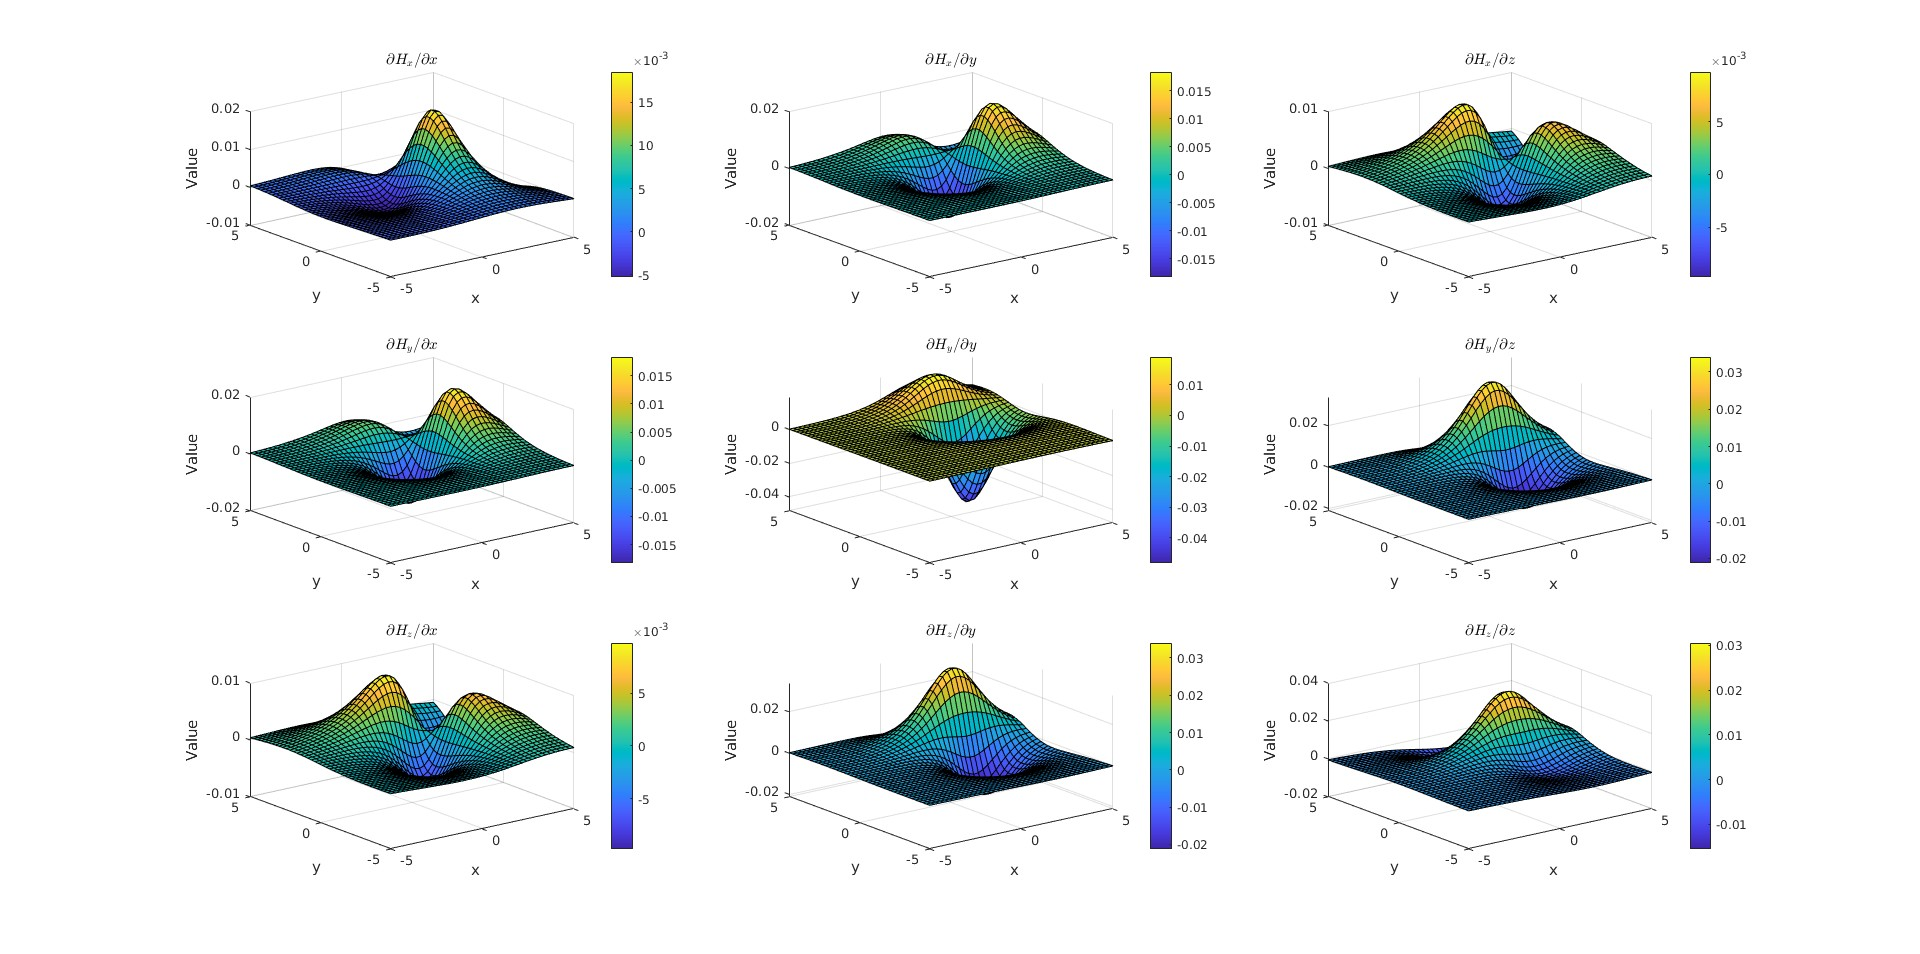
\includegraphics[width=1.4\textwidth]{images/gradients_rotated_single_anal.jpg}
\caption{Plot of the gradient tensor $\mathbf{G}$ elements
when computed analytically after the position of the signle source is translated to $(2,2,0)$ and an 
introduction of the different roations, expressed using $\mathbf{R}^t_r$ and $\mathbf{R}_t^g$.}
\label{fig:gradients_rotated_single_anal}
\end{figure}
\begin{figure}
    \centering
    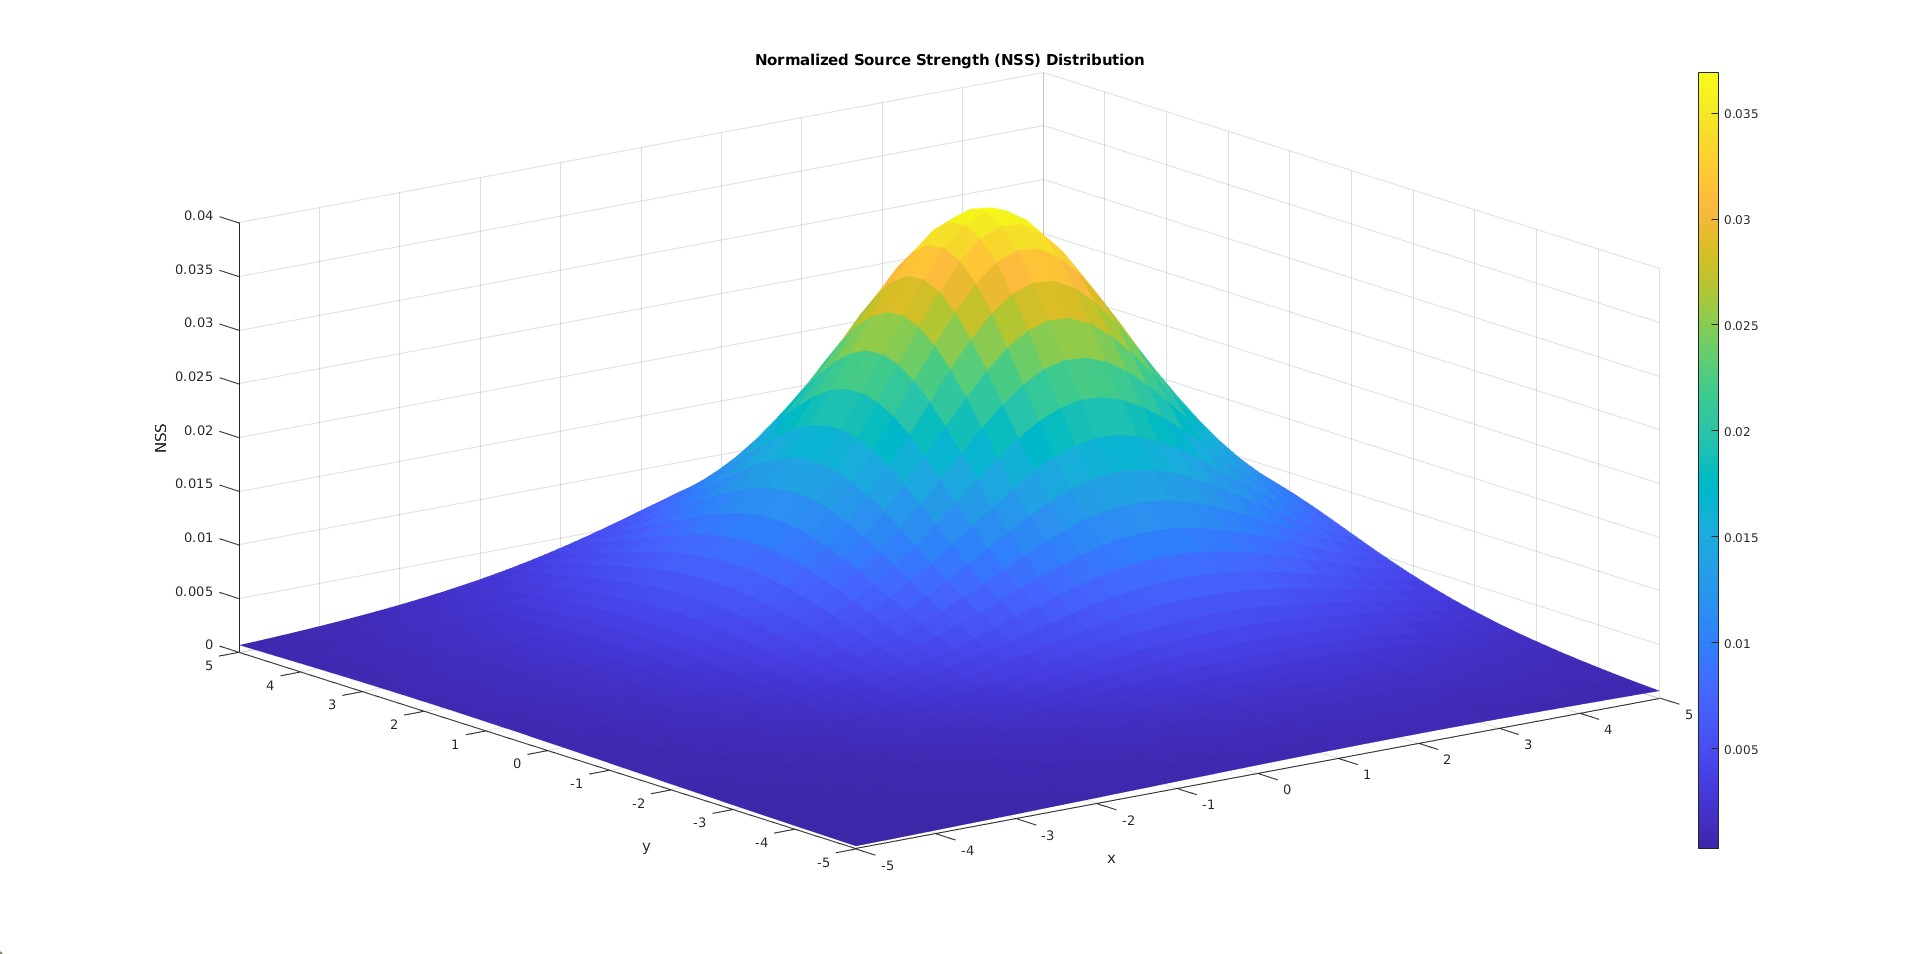
\includegraphics[width=0.8\textwidth]{images/NSS_rotated_single_anal.jpg}
    \caption{Plot of the NSS computed analytically after the position of the signle source is translated to $(2,2,0)$ and 
    different roations are introduced, expressed using $\mathbf{R}^t_r$ and $\mathbf{R}_t^g$.}
    \label{fig:NSS_rotated_single_anal}
\end{figure}

\subsubsection{Central difference method}
We also simulate and compare another method to find the gradient tensor matrix
${}^r \mathbf{G}$, which comes closer to a real world scenario.
We call this method numerical and it consists of obtaining the 
signal measured by the instrument, which is the electromagnetic field intensity
${}^r \mathbf{H}$, and then compute directly its relative gradient tensor using a 
numerical approximation.
We simulate and simplify the way the authors of \cite{NSS_single_localization} use 
a cubic structure measurement array composed of eight
TAMs\footnote{TAM stands for Tri-Axial Magnetometer} in order to obtain the magnetic
field information and then compute the gradient tensor ${}^r \mathbf{G}$.

\noindent
\\
In order to numerically compute the gradient of a 3D vector field $ \mathbf{H}( \mathbf{p}): \mathbb{R}^3 \to \mathbb{R}^3$,
we apply the central difference method approximation.
Note that we omit the superscript associated with the transmitter frame \( F_t \), 
as we are referring to a general vector field in Cartesian space. In our scenario, however, 
we have \( \mathbf{p} = {}^t \mathbf{p}_{tr} \), whose coordinates are \( (x, y, z) \).
As seen before, the gradient matrix $ \mathbf{G}$ is a \(3 \times 3\) matrix
and its $(i,j)$th entry is $G_{ij} = \partial H_i / \partial q_j$, therefore
remembering the definition of gradient as column vector \ref{eq:nabla}, we can write the gradient tensor as:
\begin{equation}
 \mathbf{G} =
\begin{bmatrix}
\frac{\partial \mathbf{H}}{\partial x} \\
\frac{\partial \mathbf{H}}{\partial y} \\
\frac{\partial \mathbf{H}}{\partial z}
\end{bmatrix}
=
\begin{bmatrix}
    \nabla H_x &
    \nabla H_y &
    \nabla H_z
\end{bmatrix}
\end{equation}

Let's consider a small perturbation $\delta$, which perturbs the magnetic field intensity $\mathbf{H}$ in every 
coordinate direction, for all the components $H_i$ of the vector field. Then, the partial derivative of $\mathbf{H}$ with 
respect to a coordinate \( q_j \) is given by:
\begin{equation}
\frac{\partial \mathbf{H}}{\partial q_j} (\mathbf{p}) \approx \frac{\mathbf{H}(\mathbf{p} + \delta \mathbf{e}_j) 
- \mathbf{H}(\mathbf{p} - \delta \mathbf{e}_j)}{2\delta}
\label{eq:G_num}
\end{equation}

where \( \mathbf{e}_j \) denotes the unit vector in the \( j \)-th direction. The gradient matrix, 
\( \mathbf{G} \), is constructed by repeating this process for each coordinate direction.
The \( j \)-th row of \( \mathbf{G} \) is:
\begin{equation}
\mathbf{G}_j = \frac{\partial \mathbf{H}}{\partial q_j} (\mathbf{p}) = 
\nabla^\top H_i (\mathbf{p})
\label{eq:G_completa}
\end{equation}

\begin{figure}
\centering
\hspace*{-0.2\textwidth}
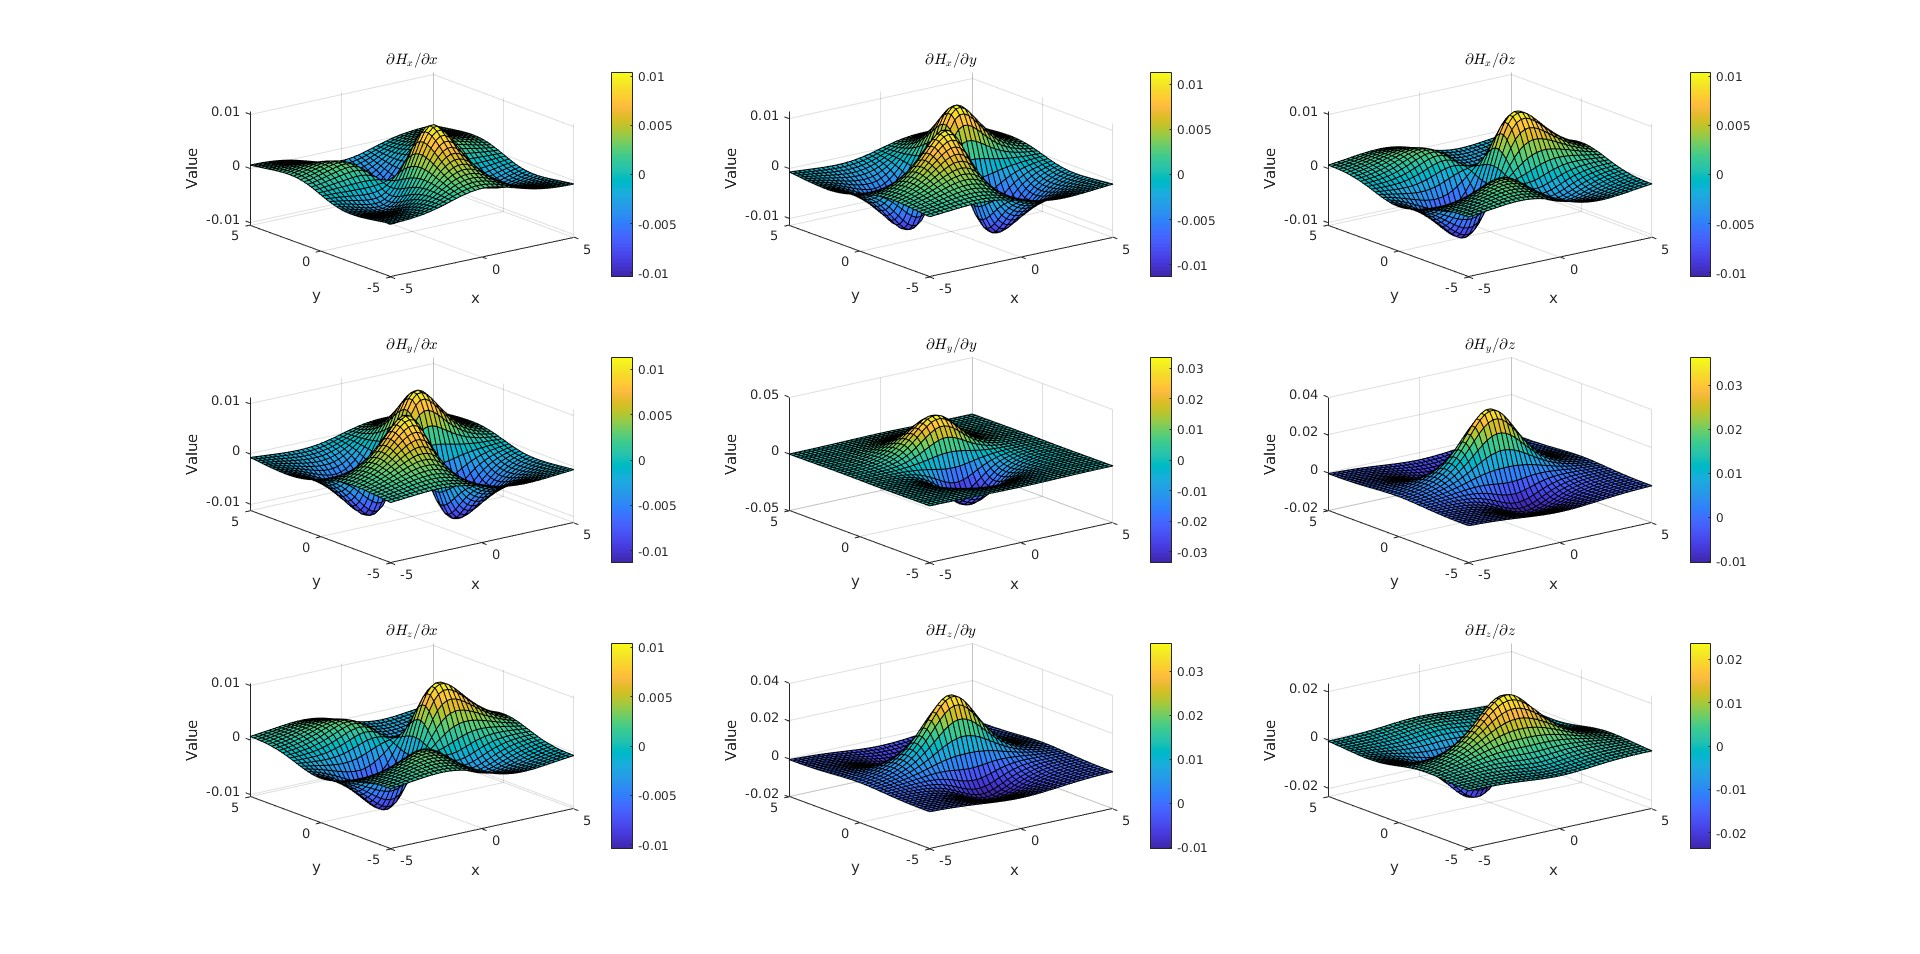
\includegraphics[width=1.4\textwidth]{images/gradients_single_num.jpg}
\caption{Plot of the gradient tensor \( \mathbf{G} \) elements
when computed numerically as in \eqref{eq:G_num}, for a single source located
at the center \( (0,0,0) \) of the space, with no rotations between the coordinate
frames \( F_g \), \( F_r \), and \( F_t \).}
\label{fig:gradients_single_num}
\end{figure}

In Figure \ref{fig:gradients_single_num}, we show the results obtained by computing the 
gradient tensor \( \mathbf{G} \) numerically, compared to the analytical method, 
for the case where there are no rotations between reference frames, and the source is located 
at the origin. We computed the difference between the gradient tensor matrices 
in the analytical and numerical cases, \( \Delta \mathbf{G} = \mathbf{G}_{\text{analytical}} - \mathbf{G}_{\text{numerical}} \), 
and calculated the Frobenius norm  \ref{eq:frobenius} of the difference matrix at all points \( \mathbf{p} \) in space.
The error was found to be on the order of \( 10^{-13} \), indicating a very accurate approximation.
The Frobenius norm is given by the square root of the sum of the squared elements \( \delta H_{ij} \) 
of the difference matrix \( \Delta \mathbf{G} \):
\begin{equation}
    \|\Delta \mathbf{G}\|_F = \sqrt{\sum_{i=1}^3 \sum_{j=1}^3 |\Delta H_{ij}|^2}
    \label{eq:frobenius}
\end{equation}
For conciseness, we omit the plot of the NSS since it remains the same, 
as the gradients did not change.
    
\noindent
\\
Next, we need to verify that the gradient tensor matrix remains symmetric under 
rototranslations of the coordinate frames and that the NSS value also remains invariant.
In particular, we apply the following transformations to each point $\mathbf{p}$ in space:
firstly we express $\mathbf{p}$ in the transmitter frame using \ref{eq:pt}, which we denoted as 
${}^t \mathbf{p}_{tr}$.
Then we apply rotation $\mathbf{R}^t_r$ to obtain the point expressed in the receiver coordinates:
\begin{equation}
   {}^r \mathbf{p}_{tr}  = \mathbf{R}^t_r \, {}^t \mathbf{p}_{tr}
   \label{eq:p__in_receiver}
\end{equation}
Now, we perturb ${}^r \mathbf{p}_{tr}$ by $\delta$ positively and negatively, in the receiver frame:
\[
\begin{cases}
    {}^r \mathbf{p}_{tr} + \delta \mathbf{e}_j \\
    {}^r \mathbf{p}_{tr} - \delta \mathbf{e}_j
\end{cases} 
\quad \text{where } j \in \{ x_r, y_r, z_r \} \, \text{relative to the coordinate frame } F_r.
\]
We find the perturbed magnetic field intensity in the transmitter frame using Eq. \ref{eq:final_H}:
${}^t \mathbf{H} ( {\mathbf{R}^t_r}^\top ({}^r \mathbf{p}_{tr} \pm \delta \mathbf{e}_j) )$.
Therefore, we are now able to find the perturbed magnetic field intensity in the receiver frame
${}^r \mathbf{H}$ and apply the central difference approximation 
\ref{eq:G_num} to compute the gradient tensor in the receiver reference frame 
${}^r \mathbf{G}$:
\begin{equation}
    \frac{\partial \mathbf{H}}{\partial q_j} = 
    \frac{
    \mathbf{R}^t_r \, {}^t \mathbf{H} ( {\mathbf{R}^t_r}^\top ({}^r \mathbf{p}_{tr} + \delta \mathbf{e}_j) )
    - \mathbf{R}^t_r \, {}^t \mathbf{H} ( {\mathbf{R}^t_r}^\top ({}^r \mathbf{p}_{tr} - \delta \mathbf{e}_j) )}
    {2 \delta}
\end{equation}
where $j \in \{ x_r, y_r, z_r \}$ as before.

\noindent
Finally, we obtained the rows of ${}^r \mathbf{G}$ and using Eq.\ref{eq:G_completa}, 
we obtain the complete gradient matrix. Then we can compute the eigenvalues and the NSS
with Eq. \ref{eq:NSS}.

\begin{figure}
\centering
\hspace*{-0.2\textwidth}
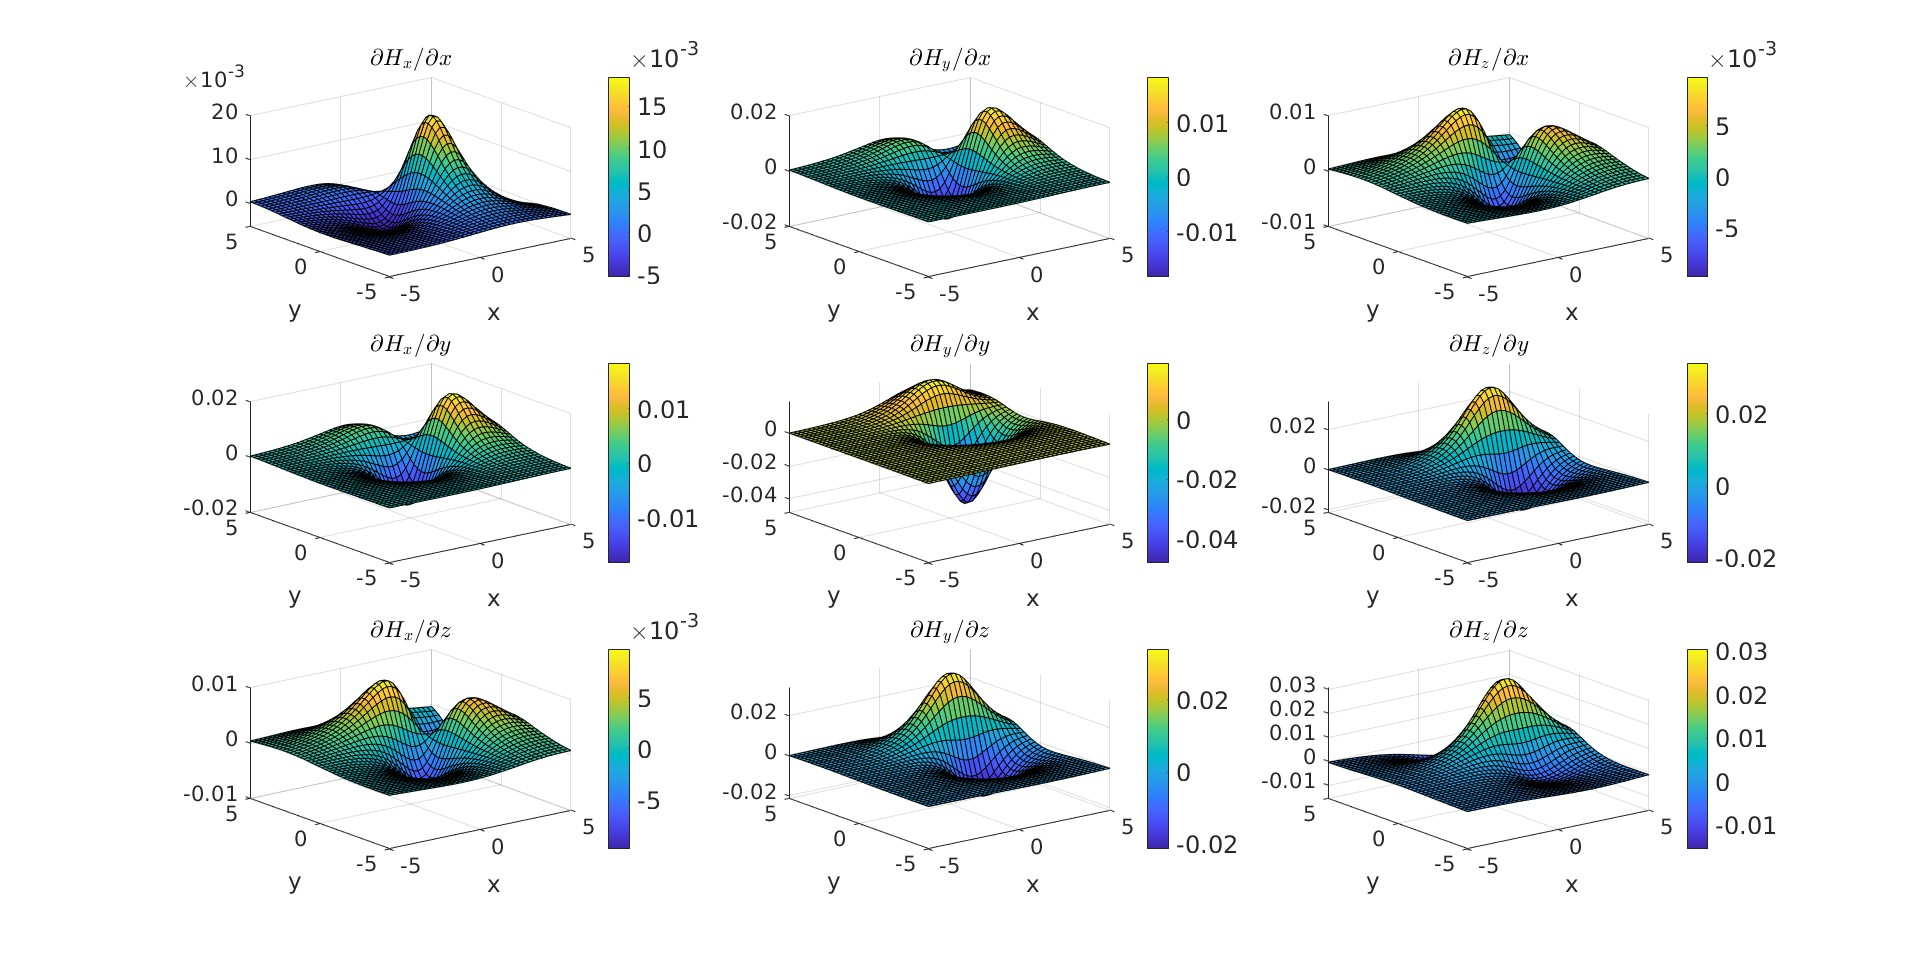
\includegraphics[width=1.4\textwidth]{images/gradients_rotated_single_num.jpg}
\caption{Plot of the gradient tensor ${}^r \mathbf{G}$ elements
when computed numerically after the position of the single source is translated to $(2,2,0)$ and an 
introduction of the different rotations, expressed using $\mathbf{R}^t_r$ and $\mathbf{R}_t^g$.}
\label{fig:gradients_rotated_single_num}
\end{figure}
\begin{figure}
\centering
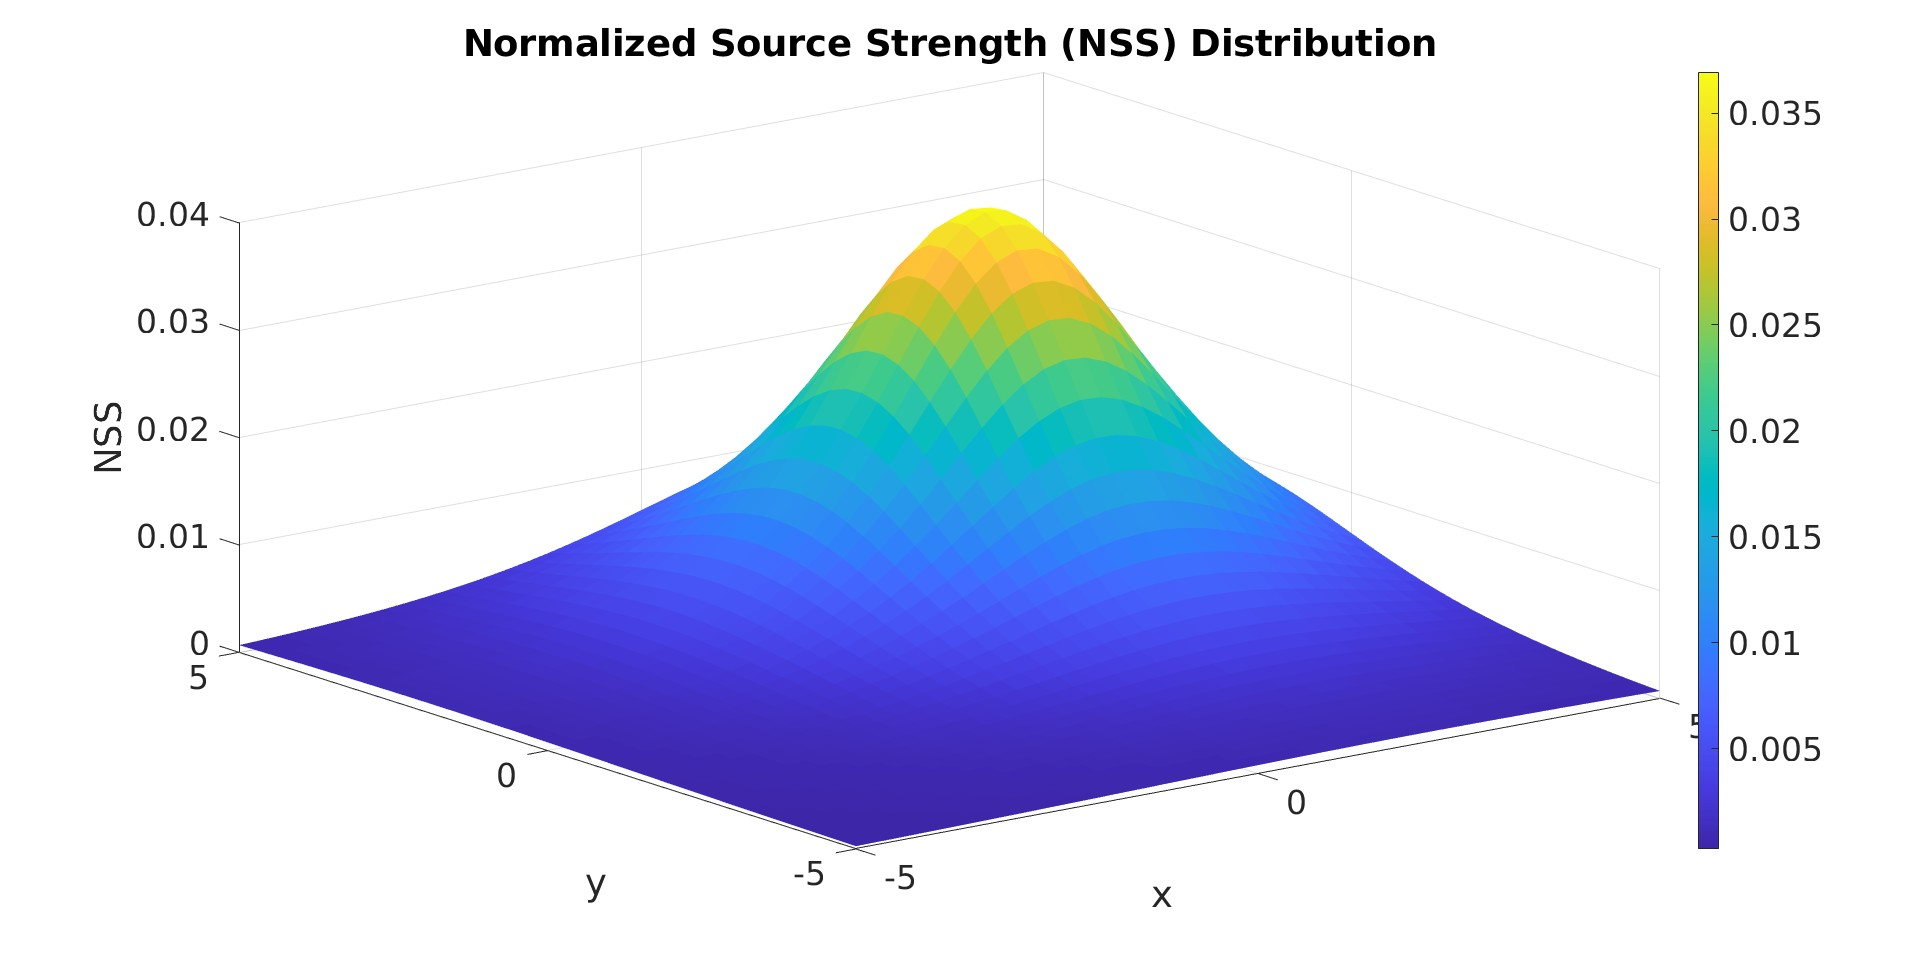
\includegraphics[width=0.8\textwidth]{images/NSS_rotated_single_num.jpg}
\caption{Plot of the NSS computed numerically, after the position of the signle source is translated to $(2,2,0)$ and 
different roations are introduced, expressed using $\mathbf{R}^t_r$ and $\mathbf{R}_t^g$.}
\label{fig:NSS_rotated_single_num}
\end{figure}

\noindent
\\
In Figure \ref{fig:gradients_rotated_single_num}, we see that we obtain the same 
gradient tensor matrix at all points in space like in the analytical approach, and therefore 
we verify that it respects the symmetry property.
Naturally, the computed NSS remains unchanged as well, as we show in Fig.~\ref{fig:NSS_rotated_single_num}.

\newpage
\section{Multiple Victims Case}
%https://math.stackexchange.com/questions/4761965/addition-of-vectors-in-different-coordinate-systems
%https://www2.physics.ox.ac.uk/sites/default/files/2011-10-08/coordinates_pdf_51202.pdf
\begin{figure}[H]
    \centering
    \tdplotsetmaincoords{70}{110}
    \begin{tikzpicture}[tdplot_main_coords]
    \draw[thick,->] (0,0,0) -- (1,0,0) node[anchor=north east]{$y_g$};
    \draw[thick,->] (0,0,0) -- (0,1,0) node[anchor=north west]{$z_g$};
    \draw[thick,->] (0,0,0) -- (0,0,1) node[anchor=south]{$x_g$};
    % Point Pt1
    \coordinate (Pt1) at (5,0,5);
    \draw[->, thick] (0,0,0) -- (Pt1) node[pos=0.5,anchor= west]{$\mathbf{p}_{t_1}$};
    % pr
    \draw[->, thick] (0,0,0) -- (p1) node[pos=0.5,anchor=west]{$\mathbf{p}_r$};
    % Point Pt2
    \coordinate (Pt2) at (0,5,3);
    \draw[->, thick] (0,0,0) -- (Pt2) node[pos=0.5,anchor= south]{$\mathbf{p}_{t_2}$};
    % Point t1p
    \coordinate (p1) at (5,5,6);
    \draw[->, thick] (5,0,5) -- (p1) node[pos=0.5, anchor=south]{$\stackrel{t_1}{\phantom{p}\bm{p}}$};      
    \node at (p1) [anchor=south] {$\bm{p}$};    
    % Point t2p
    \coordinate (p2) at (5,5,6);
    \draw[->, thick] (0,5,3) -- (p2) node[pos=0.5, anchor=south]{$\stackrel{t_2}{\phantom{p}\bm{p}}$};
    \node at (p2) [anchor=south] {$\bm{p}$};
    % Vectors H1 and H2
    \coordinate (H1) at (3,1.5,3); 
    \coordinate (H2) at (1,3,3); 
    \draw[->, thick, blue] (p1) -- (H1) node[anchor=north west]{$\mathbf{H}_1$};
    \draw[->, thick, red] (p1) -- (H2) node[anchor=north]{$\mathbf{H}_2$};
    % Angle arc
        \pic ["$\alpha$",draw = black, ->,
        angle radius=7mm,
        angle eccentricity=1.3, 
        ] { angle = H1--p1--H2};
    \coordinate (Shift) at (5,0,5);
    \tdplotsetrotatedcoordsorigin{(Shift)}
    \draw[thick,tdplot_rotated_coords,->] (0,0,0) --
    (.7,0,0) node[anchor=north]{$y_{t_1}$};
    \draw[thick,tdplot_rotated_coords,->] (0,0,0) --
    (0,.7,0) node[anchor=west]{$z_{t_1}$};
    \draw[thick,tdplot_rotated_coords,->] (0,0,0) --
    (0,0,.7) node[anchor=south]{$x_{t_1}$};
    \coordinate (Shift) at (0,5,3);
    \tdplotsetrotatedcoordsorigin{(Shift)}
    \draw[thick,tdplot_rotated_coords,->] (0,0,0) --
    (.7,0,0) node[anchor=north]{$y_{t_2}$};
    \draw[thick,tdplot_rotated_coords,->] (0,0,0) --
    (0,.7,0) node[anchor=west]{$z_{t_2}$};
    \draw[thick,tdplot_rotated_coords,->] (0,0,0) --
    (0,0,.7) node[anchor=south]{$x_{t_2}$};
    \end{tikzpicture}
    \caption{Only 2 victims case}
    \label{fig:frames-2victim}
\end{figure}
In the case of multiple victims, an ARTVA transmitter is attached to each
avalanche victim and emits an electromagnetic field. Consequently, the signal received 
by each drone (receiver) is a superposition of the effects of the multiple 
electromagnetic sources. In addition, each source has a uniquely oriented
body frame, which we will denote with $ F_{t_i}$, 
where \( i = 1, 2, \dots, n \) and \( n \in \mathbb{N} \) is the total number of sources.
In addition, we also define the global (inertial) frame $F_g$ and the receiver frame relative to the
each drone $F_r$, in the same way as the single victim case.
Then, the relative position of the receiver with respect to each trasmitter 
${}^{t_i} \mathbf{p}_{{t_i}r}$ is denoted by ${}^{t_i} \mathbf{p}$, for semplicity;
and the position of the $i$-th source in the global frame is denoted by 
$\mathbf{p}_{t_i}$.
The relative orientation of frames $F_{t_1}, F_{t_2}, \dots, F_{t_n}$ with respect to 
the reference frame $F_i$ are denoted with $\mathbf{R}^g_{t_i} \in \textit{SO}(3)$.
Instead the rotation matrices that describe the orientation between the receiver
frame and the multiple trasmitters are defined as $\mathbf{R}^{t_i}_r \in \textit{SO}(3)$.

Then, considering the receiver drone positioned at point $\mathbf{p}$ in space, the superposition
of all the electromagnetic fields can be expressed 
as the sum of the magnetic field intensity vectors \(\mathbf{H}_n\), 
when projected in the receiver frame $F_r$, as in \cite{multiple_spacecraft}:
\begin{equation}
    {}^r \mathbf{H}_{\text{tot}} = 
    {}^r \mathbf{H}_1 + {}^r \mathbf{H}_2 + \cdots + {}^r \mathbf{H}_n 
    \label{eq:sum_H}
\end{equation}
Therefore, since the receiver is rotated with respect to each transmitter, we can rewrite it as:
\begin{equation}
    {}^r \mathbf{H}_{\text{tot}} = 
    R^{t_1}_r \, {}^{t_1} \mathbf{H}_1({}^{t_1} \mathbf{p}) + R^{t_2}_r \, {}^{t_2} \mathbf{H}_2({}^{t_2} \mathbf{p}) + \cdots + R^{t_n}_r \, {}^{t_n} \mathbf{H}_n({}^{t_n} \mathbf{p})
\label{eq:sum_H_rotated}
\end{equation}
Remembering Eq.\ref{eq:H_spheric}, we can express each single magnetic field intensity vector generated
by the \(i\)-th magnetic source as:
\[
{}^{t_i} \mathbf{H}_i = \frac{I b^2}{4\pi r^3} \left( \mathbf{e}_{r_i} \, 2 \cos \theta + \mathbf{e}_{\theta_i} \, \sin \theta \right)
\]
Furthermore, we use the same homogeneous transformation as in the single victims case, Eq.\ref{eq:pt}:
\begin{equation}
    \mathbf{p}_{t_i} + R^g_{t_i} \, {}^{t_i} \mathbf{p} = \mathbf{p}_r
    \label{eq:pt_multi}  
\end{equation}
which is again inverted:
\begin{equation}
    {}^{t_i} \mathbf{p} = {R^g_{t_i}}^\top \, \left( \mathbf{p}_r - \mathbf{p}_{t_i} \right)
    \label{eq:pt_transmitter}
\end{equation}
In Figure \ref{fig:frames-2victim}, for clarity, we represent all the frames described before, 
in the case of only two victims.
 

\subsection{Total Magnitude}
In the multiple victims case, the use of the total magnitude of the magnetic
field intensity $|| \mathbf{H} ||$ as a mean to infer the position of
the multiple sources, is an unfeasible strategy.
In this section, we motivate the rationale behind our reasoning, by obtaining
the mathematical formula of the total magnitude.
Specifically, we aim to demonstrate that, even after the use of the previous 
approximation \ref{eq:approx}, the total magnitude is highly non-linear and 
non-invertible (not even partially bijective).

\noindent
In both the single-victim and multiple ones scenarios, the orientation of the receiver frame 
relative to the transmitter frame did not affect the magnitude of the magnetic 
field intensity.
This is because the magnitude of any vector field (having the same 
properties of any vector quantity) is rotationally invariant.
Supposing only one source, the projection of the electromagnetic field intensity on the receiver frame is ${}^r\mathbf{H}$,
and it is related to ${}^t \mathbf{H}$ in Eq.\ref{eq:H_receiver}; then 
using simple linear algebra definitions we can write:
\begin{equation}
\|{}^r\mathbf{H}\|^2 = \|\mathbf{R}^t_r \, {}^t\mathbf{H}\|^2 = 
(\mathbf{R}^t_r \, {}^t\mathbf{H}) \cdot (\mathbf{R}^t_r \, {}^t\mathbf{H}) = 
{}^t\mathbf{H}^\top \, {\mathbf{R}^t_r}\mkern-2mu^\top \, \mathbf{R}^t_r \, {}^t\mathbf{H} = 
{}^t\mathbf{H}^\top \, {}^t\mathbf{H} = \|{}^t\mathbf{H}\|^2
\label{eq:magnitude_invariant}
\end{equation}
This shows that the magnitude of the vector field expressed in the receiver 
coordinate frame $F_r$ is equal to the one expressed in the trasmitter frame $F_t$.

\noindent
In the multiple vicims case, the receiver frame is oriented in a different way
for each one of the $n$ trasmitter ones. However, the total magnitude is still unaffected by the 
different rotations, thanks to the result we have just obtained from Eq. \ref{eq:magnitude_invariant}.
Let's suppose, for simplicity, the case of only two sources like in Figure \ref{fig:frames-2victim}.
We want to find the total magnitude of the magnetic field intensity in Eq. \ref{eq:sum_H_rotated}.
Therefore, we apply the law of cosines from linear algebra:
\[
|| \mathbf{H}_{\text{tot}}||^2 = ||{}^r \mathbf{H}_1||^2 + ||{}^r \mathbf{H}_2||^2 + 2 \, ||{}^r\mathbf{H}_1|| \, ||{}^r\mathbf{H}_2|| \cos \alpha
\]
where \( \alpha \) is the angle between the two vectors \( \mathbf{H}_1 \) and \( \mathbf{H}_2 \) on the only plane which contains both vector fields.
To use the approximation in Eq. \ref{eq:approx}, we need to express the vector fields
in the transmitter reference frame:
\begin{align*}
\|\mathbf{H}_{\text{tot}}\|^2 = 
&\ \|\mathbf{R}^{t_1}_r \, {}^t \mathbf{H}_1\|^2 + \|\mathbf{R}^{t_2}_r \, {}^t \mathbf{H}_2\|^2  + 2 \, \|\mathbf{R}^{t_1}_r \, {}^t \mathbf{H}_1\| \, \|\mathbf{R}^{t_2}_r \, {}^t \mathbf{H}_2\| \cos \alpha \\
= &\ \|{}^t \mathbf{H}_1\|^2 + \|{}^t \mathbf{H}_2\|^2 + 2 \, \|{}^t \mathbf{H}_1\| \, \|{}^t \mathbf{H}_2\| \cos \alpha.
\end{align*}

\noindent
Substituting Eq.\ref{eq:H_mag_cart} of the magnetic field magnitude after the approximation, 
with the Cartesian coordinates of reference frame $F_t$:
\[
\begin{aligned}
|| \mathbf{H}_{\text{tot}}||^2 &= \left( \frac{m}{4 \pi} \right)^2 \left( \frac{(ab)^2}{b^2 \, x_1^2 + a^2 \, (y_1^2 + z_1^2)} \right)^3 
+ \left( \frac{m}{4 \pi} \right)^2 \left( \frac{(ab)^2}{b^2 \, x_2^2 + a^2 \, (y_2^2 + z_2^2)} \right)^3 + \\
& + 2 \, \cos \alpha \left( \frac{m}{4 \pi} \right)^2 \left( \frac{(ab)^2}{b^2 \, x_1^2 + a^2 \, (y_1^2 + z_1^2)} \right)^{3/2} \left( \frac{(ab)^2}{b^2 \, x_2^2 + a^2 \, (y_2^2 + z_2^2)} \right)^{3/2} = \\
&= \left( \frac{m \, (ab)^3}{4 \pi} \right)^2 \left( \left( \frac{1}{b^2 \, x_1^2 + a^2 \, (y_1^2 + z_1^2)} \right)^3 
+  \left( \frac{1}{b^2 \, x_2^2 + a^2 \, (y_2^2 + z_2^2)} \right)^3 \right. + \\
& \left. + \, 2 \, \cos \alpha \left( \frac{1}{(b^2 \, x_1^2 + a^2 \, (y_1^2 + z_1^2))(b^2 \, x_2^2 + a^2 \, (y_2^2 + z_2^2))} \right)^{3/2} \right)
\end{aligned}
\]
Note that a and b, have the same values for all the fields since they have been chosen in order to optimize the magnitude of the 
general magnetic field intensity $\mathbf{H}$. 
Also we suppose that the radius $b$ and the current $I$ are the same for all the devices (so same magnetic moment $m$).
Bringing the common terms to the left side and inverting all the fractions:
\[
\begin{aligned}
\left( \frac{m \, (a b)^3}{4 \pi \, || \mathbf{H}_{\text{tot}}||} \right)^2 &= \left( b^2 \, x_1^2 + a^2 \, (y_1^2 + z_1^2) \right)^3 + \left( b^2 \, x_2^2 + a^2 \, (y_2^2 + z_2^2) \right)^3 + \\
& + 2 \, \cos \alpha \left( (b^2 \, x_1^2 + a^2 \, (y_1^2 + z_1^2))(b^2 \, x_2^2 + a^2 \, (y_2^2 + z_2^2)) \right)^{3/2}
\end{aligned}
\]

\noindent
From this point it is not possible to carry out the mathematical operations that 
have been carried out in the single-victim case.
Therefore, it is not possible to find a mapping as in \ref{eq:mapping},
as the above equation is not even partially bijective.
Furthermore, the non-invertibility and non linearities, determined by the cross terms,
would only increase in the cases of more than two victims.
In the following section, we will describe an alternative approach, which employs the
NSS as a mean to estimate the position of multiple avalanche victims. 

\subsection{Normalized Source Strength}
As already mentioned, the properties of rotational invariance (see Eq.\ref{eq:rotational_invariance}) 
and rapid decaying of the NSS (see Eq.\ref{eq:NSS_decay}) are 
particularly beneficial in the multiple-victims case.
In this section, we will describe how we compute the gradient tensor matrix 
${}^r G_{\text{tot}}$ and the NSS in the multiple-victims case,
for a drone located at point $p$ in space with a rigidly attatched body fram $F_t$.
We employ these procedures to simulate the results over a spatial range of $[10, 10]$ meters, 
when we fix the $z$-coordinate fixed at 3 m (i.e., the \( xy \)-plane at \( z = 3 \)), 
in which three victims are positioned at \((0, 0, 0)\), \((-6, -6, 0)\), and \((7, 7, 0)\) respectively.
% The rotations are 
% R_array{1} = rotationMatrix(130, 0, 0);
% R_array{2} = rotationMatrix(0, 50, 0);  
% R_array{3} = rotationMatrix(0, 0, 140);

% R_drones{1} = rotationMatrix(90, 0, 0);
% R_drones{2} = rotationMatrix(0, 200, 0);  
% R_drones{3} = rotationMatrix(0, 0, 300);

\subsubsection{Analitycal method}
The analytical method in the multiple-victims case is similar to the single-victims one;
we will describe the general procedure when different orientations
are presentbetween the different reference frames $F_g$, $F_r$, and $F_{t_i}$.

Firstly, for each different $i$-th source we express the point at which the NSS needs to be obtained
in the transmitter reference frame $F_{t_i}$, in the same way as Eq.\ref{eq:pt_multi}.

Secondly, we use the analytical expression in Eq.\ref{eq:G_analit}, to compute the gradient tensor 
in the transmitter frame ${}^{t_i} \mathbf{G}_i$, of the $i$-th source.
Then we transform ${}^{t_i} \mathbf{G}_i$ in ${}^r \mathbf{G}_i$, the gradient expressed in the receiver frame using Eq.\ref{eq:rotated_gradient_tensor}.

Finally, we find ${}^r \mathbf{G}_{\text{tot}}$, the total gradient tensor by summing all the gradient tensors
relative to the different suorces in the common receiver frame:
\begin{align}
{}^r \mathbf{G}_{\text{tot}} &= 
\mathbf{R}^{t_1}_r  \, {}^{t_1}\mathbf{G}_1({}^{t_1} \mathbf{p}) \, {\mathbf{R}^{t_1}_r}\mkern-2mu^\top + \dots + \mathbf{R}^{t_n}_r  \, {}^{t_n}\mathbf{G}_n({}^{t_n} \mathbf{p}) \, {\mathbf{R}^{t_n}_r}\mkern-2mu^\top \nonumber = \\
&= 
\mathbf{R}^{t_1}_r  \, {}^{t_1}\mathbf{G}_1({R^g_{t_1}}\mkern-4mu^\top ( \mathbf{p}_r - \mathbf{p}_{t_1})) \, {\mathbf{R}^{t_1}_r}\mkern-3mu^\top + 
\cdots + \mathbf{R}^{t_n}_r   {}^{t_n}\mathbf{G}_n({R^g_{t_1}}\mkern-3mu^\top ( \mathbf{p}_r - \mathbf{p}_{t_1}))  {\mathbf{R}^{t_n}_r}\mkern-3mu^\top
\label{eq:G_tot}
\end{align}
Note that we sum the gradient matrices, rather than summing the 
magnetic field intensity vectors \( {}^r \mathbf{H}_i \), 
as the gradient operation is linear. 
Thanks to linearity, the gradient matrix of the sum of the vectors 
is equal to the sum of the gradient tensors.
 
%GRADIENTS ANALYTICAL NO ROTATIONS
\begin{figure}
\hspace*{-0.2\textwidth}
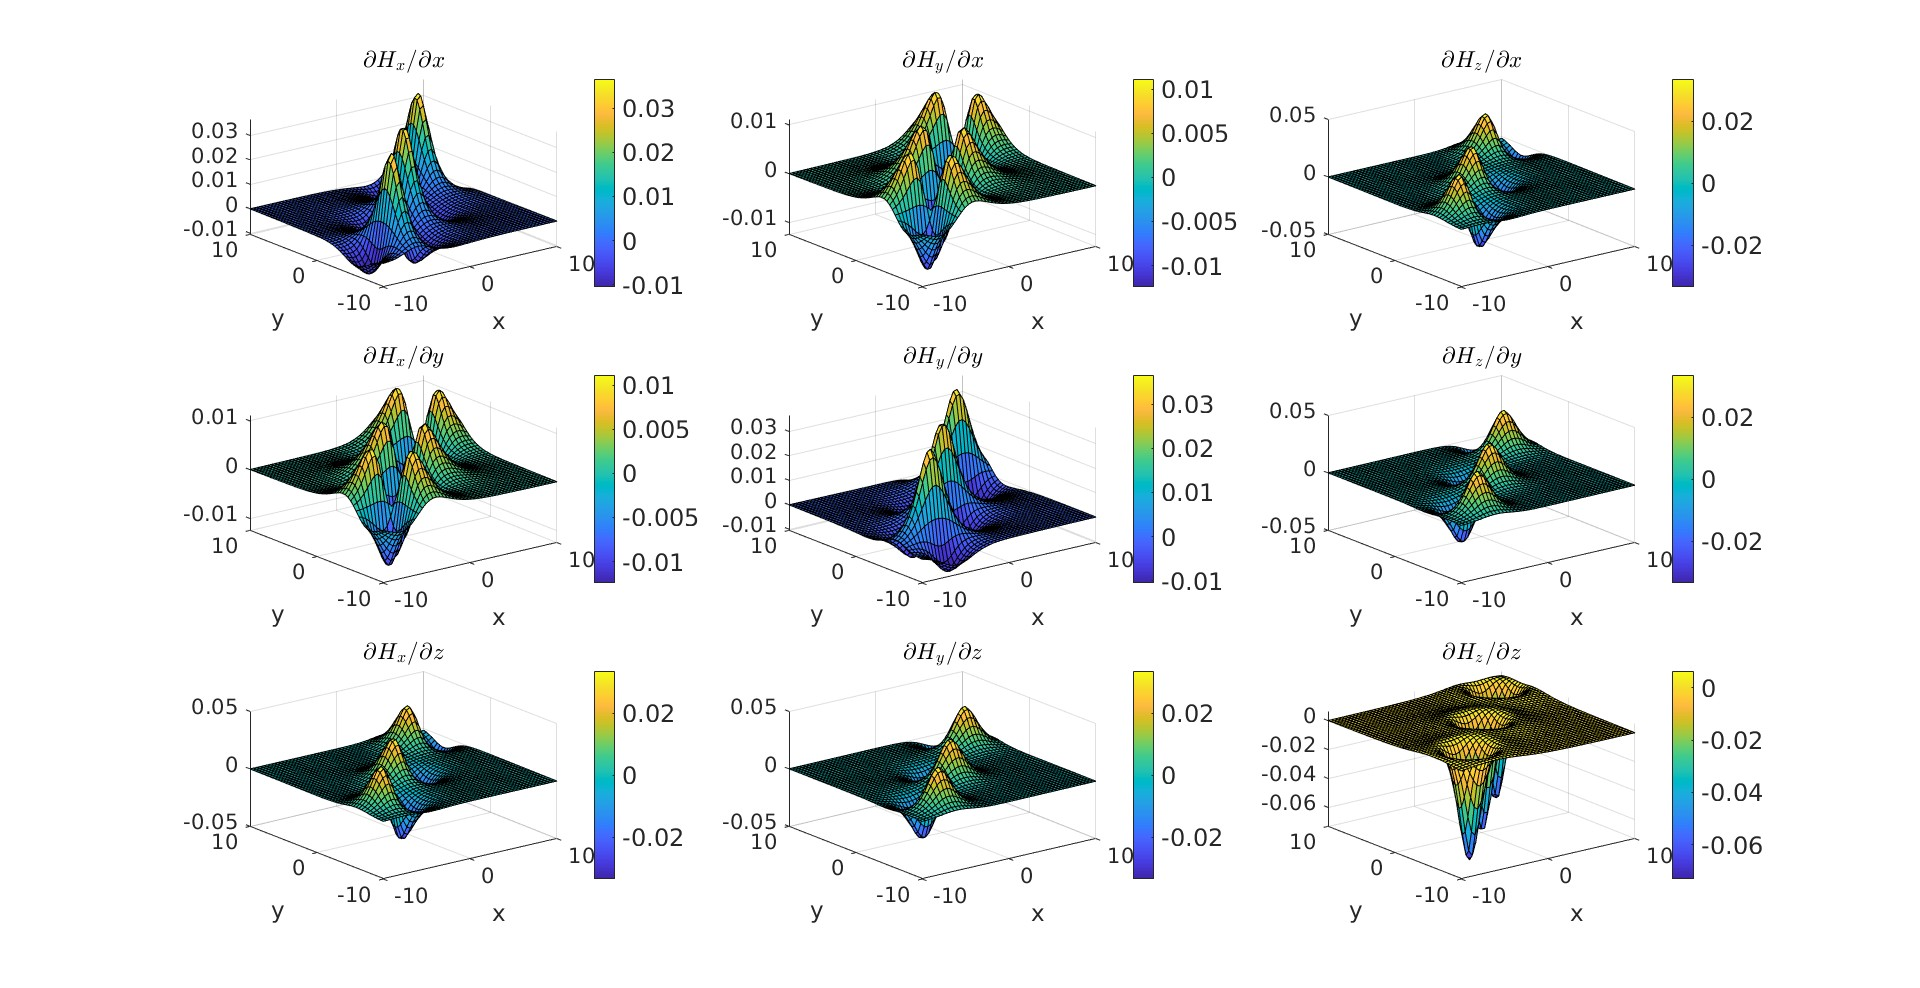
\includegraphics[width=1.4\textwidth]{images/gradients_multi_anal.jpg}
\caption{Plot of the gradient tensor ${}^r \mathbf{G}_{\text{tot}}$ elements
when computed analytically in the case of multiple sources positioned at  $(0,0,0)$, $(-6,-6,0)$, and $(7,7,0)$; with no rotations 
between the coordinate frames \( F_g \), \( F_r \), and \( F_t \).}
\label{fig:gradients_multi_anal}
\end{figure}

%NSS ANALYTICAL NO ROTATIONS
\begin{figure}
\centering
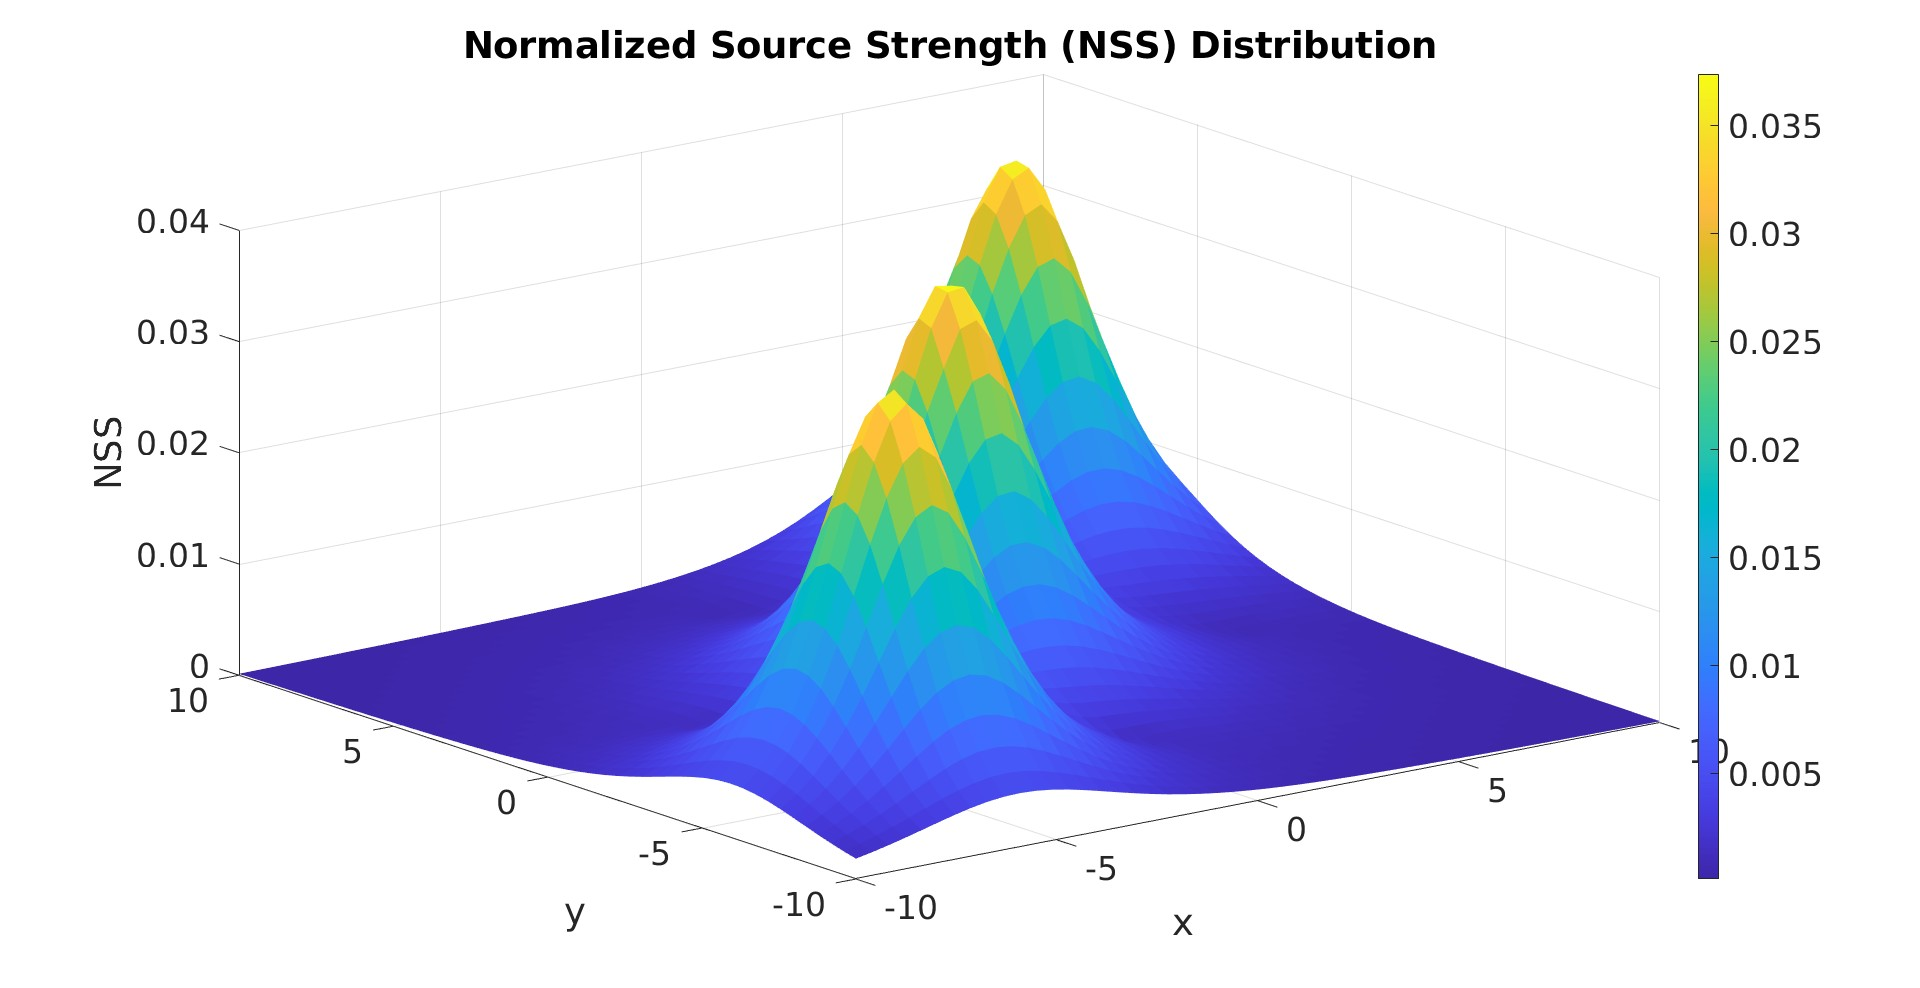
\includegraphics[width=0.8\textwidth]{images/NSS_multi_anal.jpg}
\caption{Plot of the NSS computed analytically in the case of multiple sources positioned at  $(0,0,0)$, $(-6,-6,0)$, and $(7,7,0)$; with no rotations 
between the coordinate frames \( F_g \), \( F_r \), and \( F_t \).}
\label{fig:NSS_multi_anal}
\end{figure}

%GRADIENTS ANALYTICAL ROTATIONS
\begin{figure}
\hspace*{-0.2\textwidth}
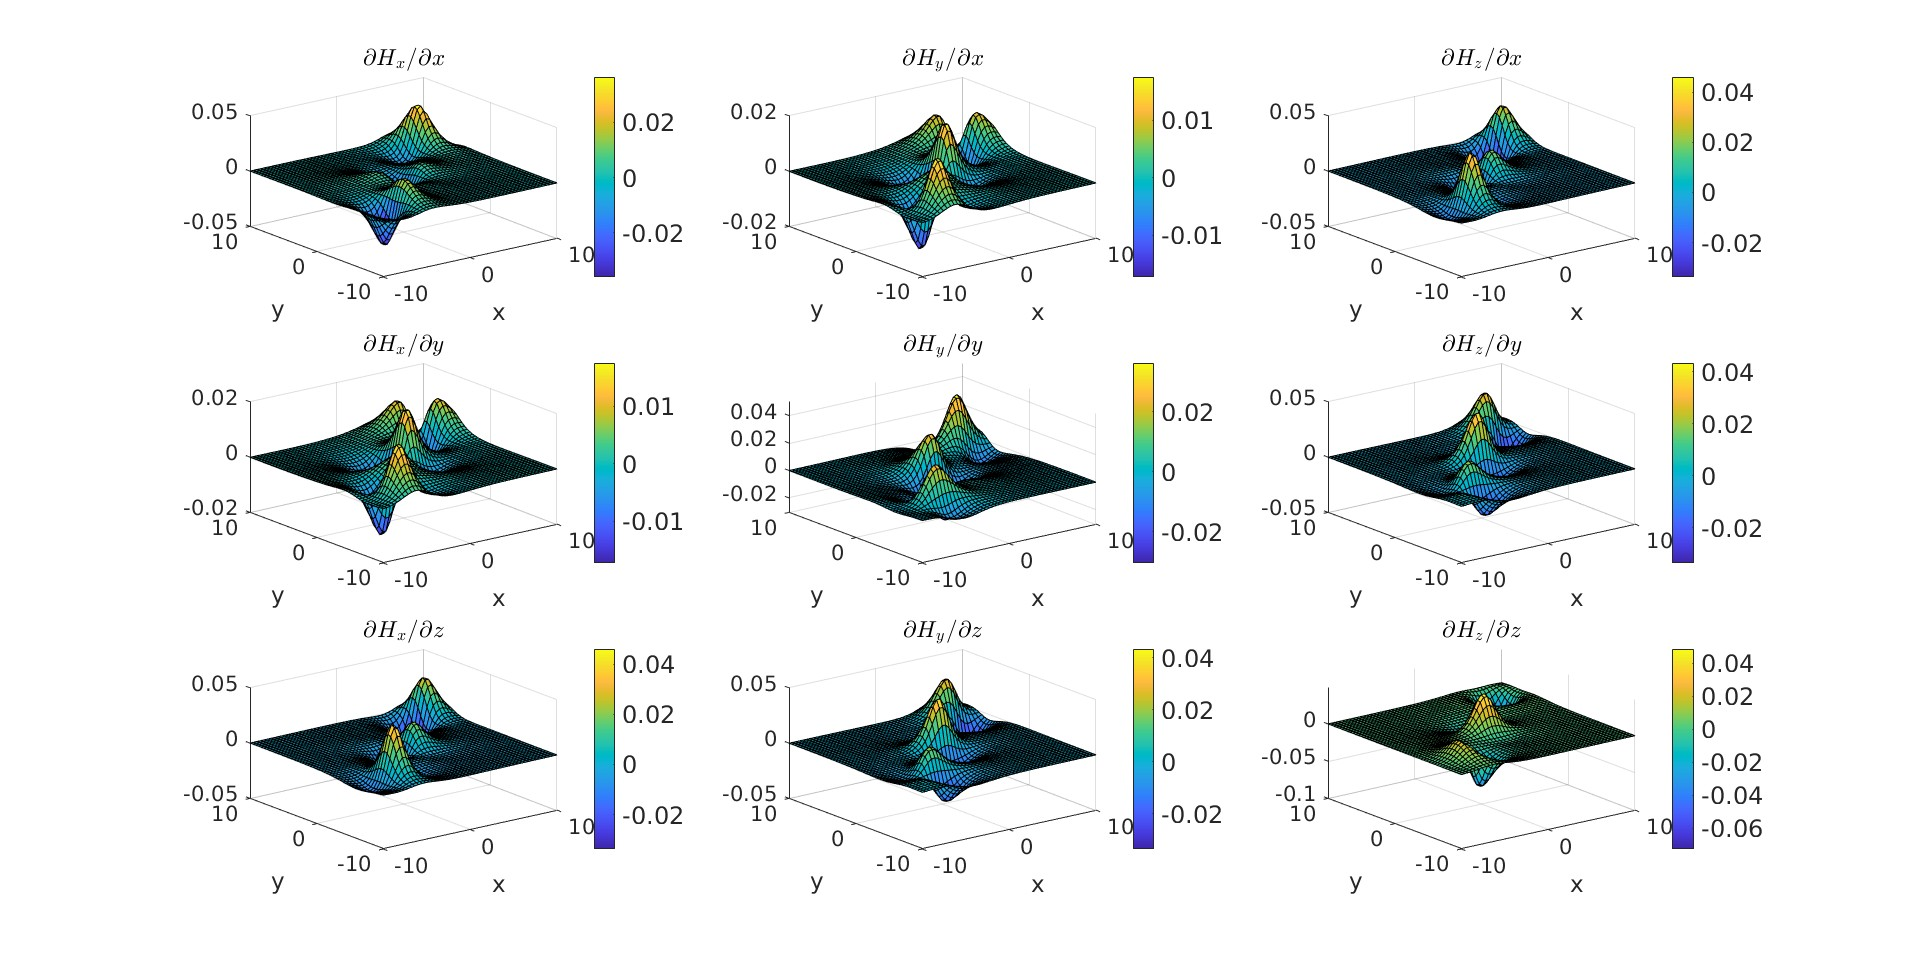
\includegraphics[width=1.4\textwidth]{images/gradients_rotated_multi_anal.jpg}
\caption{Plot of the gradient tensor ${}^r \mathbf{G}_{\text{tot}}$ elements
when computed analytically in the case of multiple sources positioned at  $(0,0,0)$, $(-6,-6,0)$, and $(7,7,0)$;
with rotations $\mathbf{R}^t_r$ and $\mathbf{R}_t^g$. }
\label{fig:gradients_rotated_multi_anal}
\end{figure}

%NSS ANALYTICAL ROTATIONS
\begin{figure}
\centering
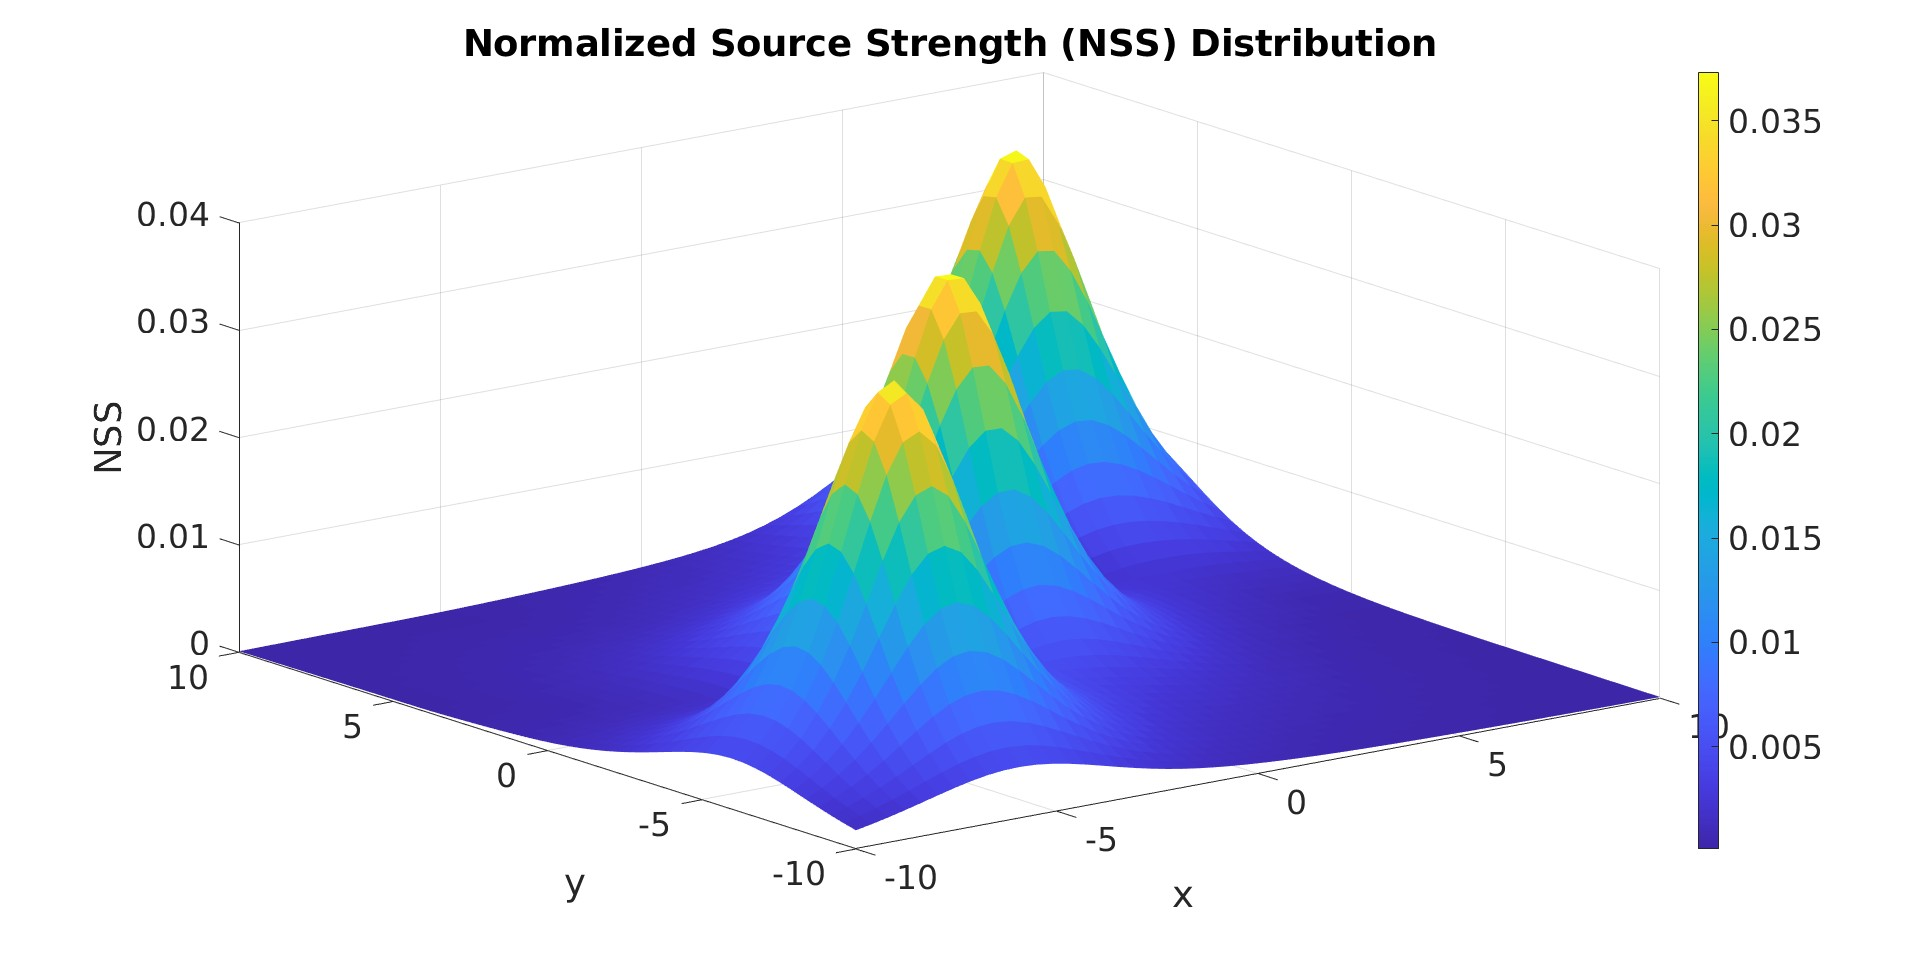
\includegraphics[width=0.8\textwidth]{images/NSS_rotated_multi_anal.jpg}
\caption{Plot of the NSS computed analytically in the case of multiple sources positioned at  $(0,0,0)$, $(-6,-6,0)$, and $(7,7,0)$;
with rotations $\mathbf{R}^t_r$ and $\mathbf{R}_t^g$.}
\label{fig:NSS_rotated_multi_anal}
\end{figure}

\noindent
By looking at Fig.\ref{fig:gradients_multi_anal} and Fig.\ref{fig:gradients_rotated_multi_anal}
we can observe that the components of the gradient matrix vary in one case with respect to another;
however the matrix mantains the symmetry property.
Instead, by comparing Fig.\ref{fig:NSS_multi_anal} with Fig.\ref{fig:NSS_rotated_multi_anal}
we verify that the NSS distribution is rotationally invariant, like in the single victims case.

\subsubsection{Numerical method}
The numerical method in the multiple-victims case is similar to the single-victims one as well;
we will describe the general procedure when different orientations
are present between the different reference frames $F_g$, $F_r$, and $F_{t_i}$.

We procede in the same way as in the analytical method: for each different $i$-th source we express the 
point at which the $k$-th UAV is localized,
in the transmitter reference frame $F_t$, Eq.\ref{eq:pt_multi}.
Then we apply rotation $\mathbf{R}^{t_i}_r$ to obtain the point expressed 
in the receiver coordinates, which we denote by ${}^r \mathbf{p}_{t_ir}$, similarly to Eq.\ref{eq:p__in_receiver}.
So that we can perturb ${}^r \mathbf{p}_{t_ir}$ by $\delta$, along each direction $j$ of the 
receiver coordinates $(x_r, y_r, z_r)$:
\[
\begin{cases}
    {}^r \mathbf{p}_{t_ir} + \delta \mathbf{e}_j \\
    {}^r \mathbf{p}_{t_ir} - \delta \mathbf{e}_j
\end{cases} 
\quad \text{where } j \in \{ x_r, y_r, z_r \} \, \text{relative to the coordinate frame } F_r.
\]
Then, to obtain the perturbed magnetic field intensity and so use Eq.\ref{eq:final_H}, we need to 
revert the last transformation and therefore we transpose the rotation matrix $\mathbf{R}^{t_i}_r$ to 
obtain the reverse transformation:
\[
\begin{cases}
    {}^{t_i} \mathbf{p}^+ = {\mathbf{R}^{t_i}_r}^\top \, ({}^r \mathbf{p}_{t_ir} + \delta \mathbf{e}_j) \\
    {}^{t_i} \mathbf{p}^- =  {\mathbf{R}^{t_i}_r}^\top \, ({}^r \mathbf{p}_{t_ir} - \delta \mathbf{e}_j) \\
\end{cases}
\]
We now have computed the perturbed magnetic field intensity vector in the transmitter frame 
generated by each one of the $i$-th source, denoted as ${}^{t_i} \mathbf{H}_i$.
Then, we rotatate each perturbed magnetic field vector to express it in the common receiver
reference frame, so that we can add the contribution of each electromagnetic field
together and obtain ${}^r \mathbf{H}_{\text{tot}}$, which is exactly what is described
in Eq.\ref{eq:sum_H_rotated}:
\[
\begin{cases}
    {}^r \mathbf{H}_{\text{tot}}^+ = 
    R^{t_1}_r \, {}^{r} \mathbf{H}_1({}^{t_1} \mathbf{p}^+)
    + \cdots + R^{t_n}_r \, {}^{t_n} \mathbf{H}_n({}^{t_n} \mathbf{p}^+) \\
    {}^r \mathbf{H}_{\text{tot}}^- = R^{t_1}_r \, {}^{r} \mathbf{H}_1({}^{t_1} \mathbf{p}^-)
    + \cdots + R^{t_n}_r \, {}^{t_n} \mathbf{H}_n({}^{t_n} \mathbf{p}^-)
\end{cases}
\]

Finally, we can find the perturbed magnetic field intensity in the receiver frame
${}^r \mathbf{H}_i$ and apply the central difference approximation 
\ref{eq:G_num} to compute the total gradient tensor in the receiver reference frame 
${}^r \mathbf{G}_{\text{tot}}$:
\begin{equation}
    \frac{\partial \mathbf{H}_{\text{tot}}}{\partial q_j} = 
    \frac{
     {}^r \mathbf{H}_{\text{tot}}^+ ({}^r \mathbf{p}_{t_1r}, \dots , {}^r \mathbf{p}_{t_nr})
    -  {}^r \mathbf{H}_{\text{tot}}^- ({}^r \mathbf{p}_{t_1r}, \dots , {}^r \mathbf{p}_{t_nr})}
    {2 \delta}
\end{equation}

\noindent
Finally, we obtained the rows of ${}^r \mathbf{G}_{\text{tot}}$ and using Eq.\ref{eq:G_completa}, 
we obtain the complete gradient matrix. Then, we can compute the eigenvalues and the NSS
with Eq.\ref{eq:NSS}, in the same way as the single-victim case.

%GRADIENTS NUMERICAL NO ROTATIONS
\begin{figure}
\hspace*{-0.2\textwidth}
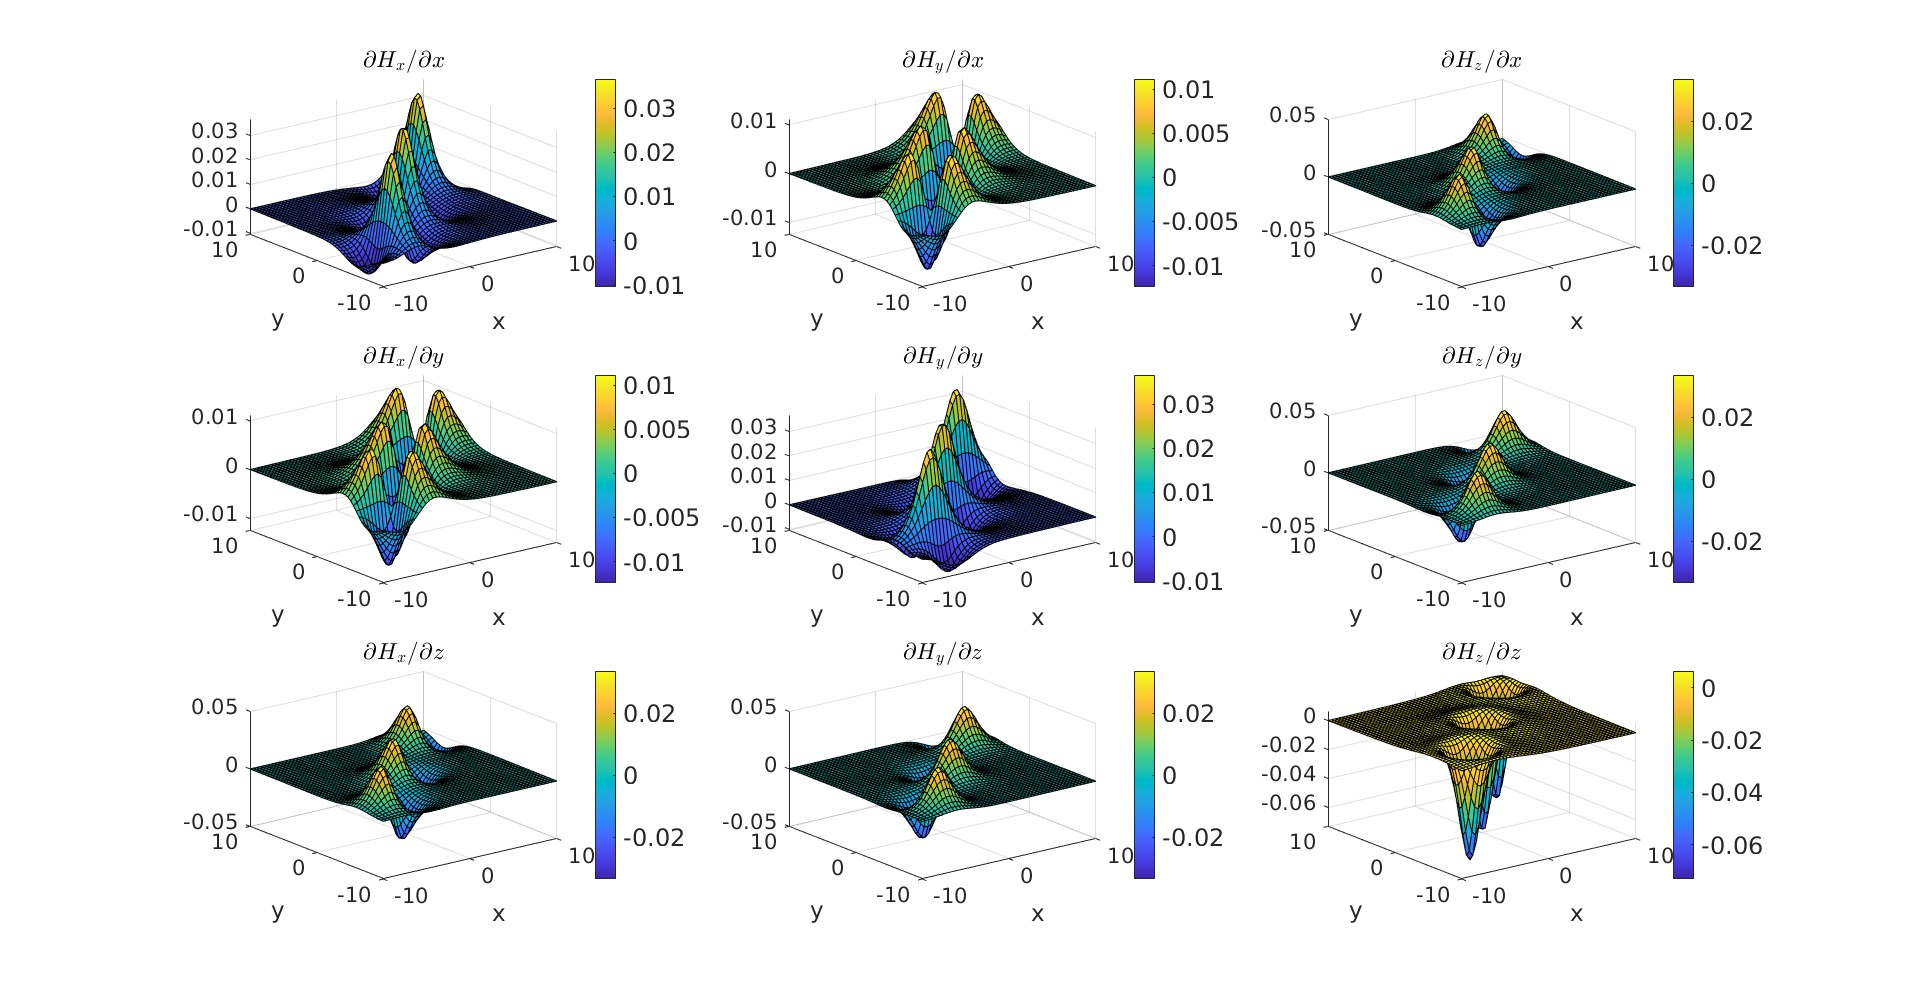
\includegraphics[width=1.4\textwidth]{images/gradients_multi_num.jpg}
\caption{Plot of the gradient tensor ${}^r \mathbf{G}_{\text{tot}}$ elements
when computed numerically in the case of multiple sources positioned at  $(0,0,0)$, $(-6,-6,0)$, and $(7,7,0)$; with no rotations 
between the coordinate frames \( F_g \), \( F_r \), and \( F_t \).}
\label{fig:gradients_multi_num}
\end{figure}

%NSS NUMERICAL NO ROTATIONS 
\begin{figure}
\centering
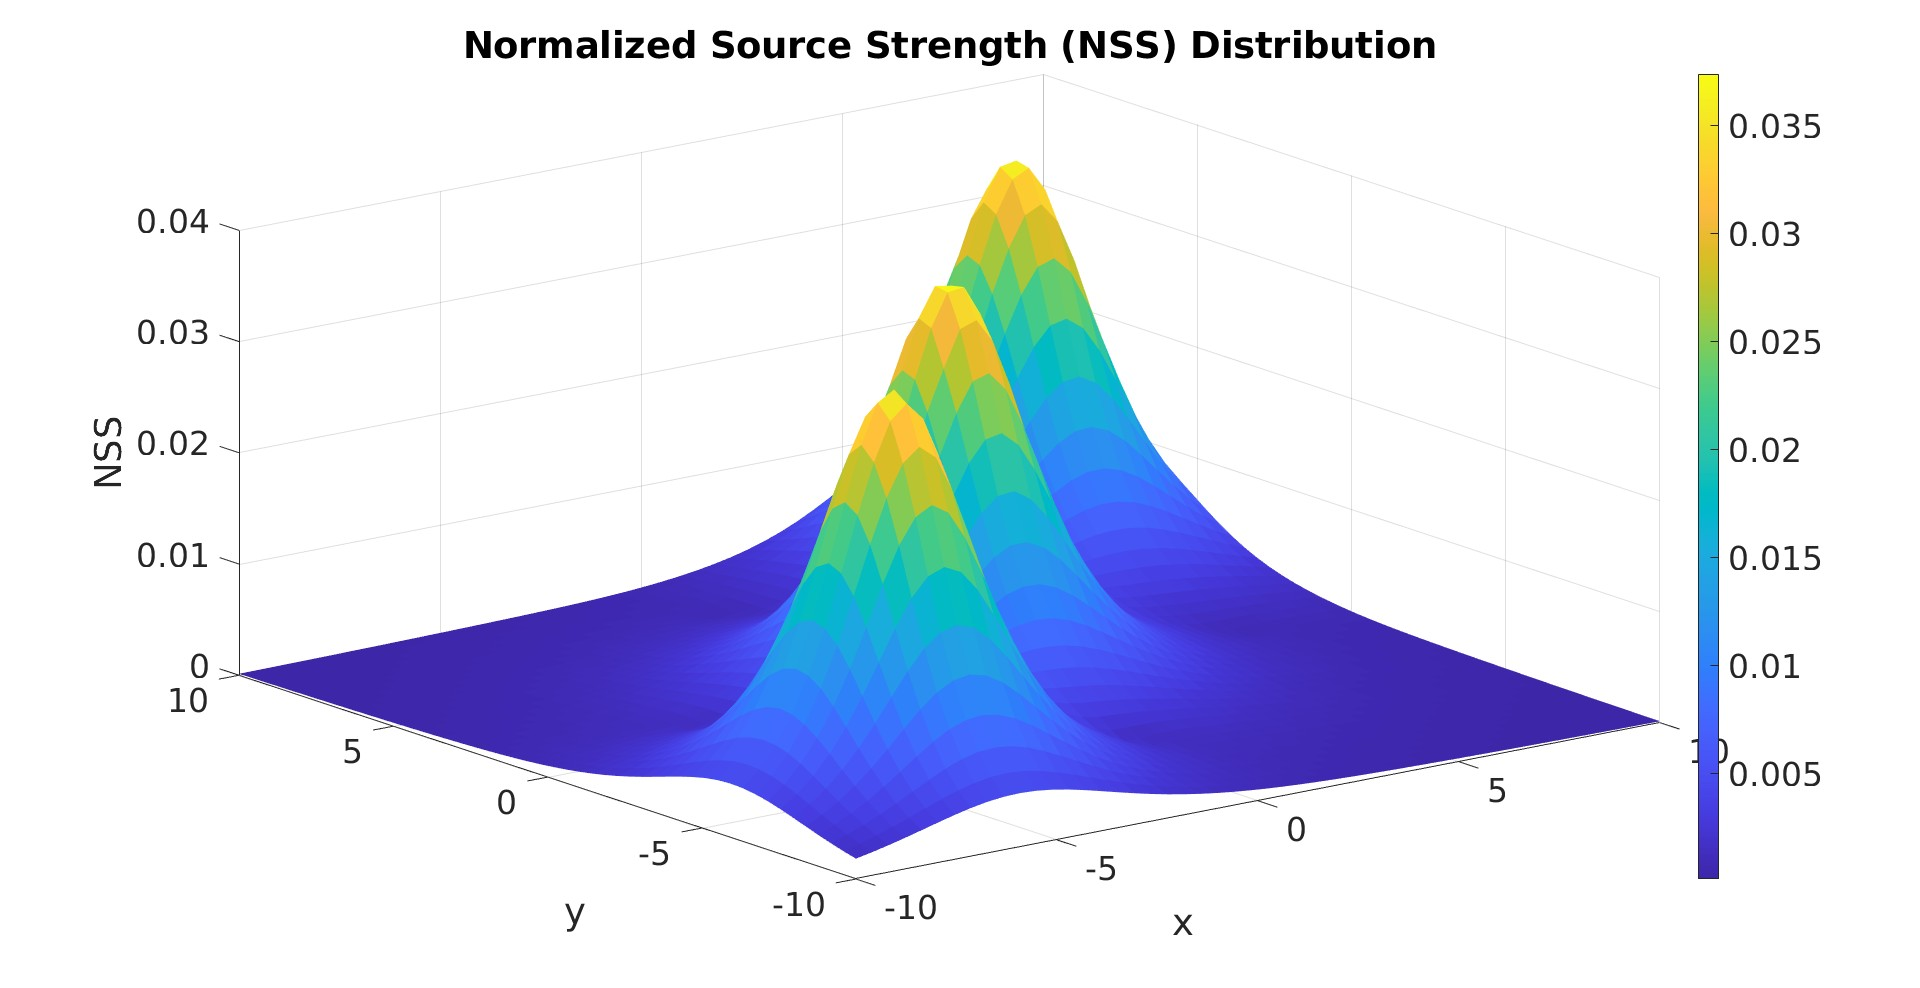
\includegraphics[width=0.8\textwidth]{images/NSS_multi_num.jpg}
\caption{Plot of the NSS computed numerically in the case of multiple sources positioned at  $(0,0,0)$, $(-6,-6,0)$, and $(7,7,0)$; with no rotations 
between the coordinate frames \( F_g \), \( F_r \), and \( F_t \).}
\label{fig:NSS_multi_num}
\end{figure}

%GRADIENTS NUMERICAL ROTATIONS
\begin{figure}
\hspace*{-0.2\textwidth}
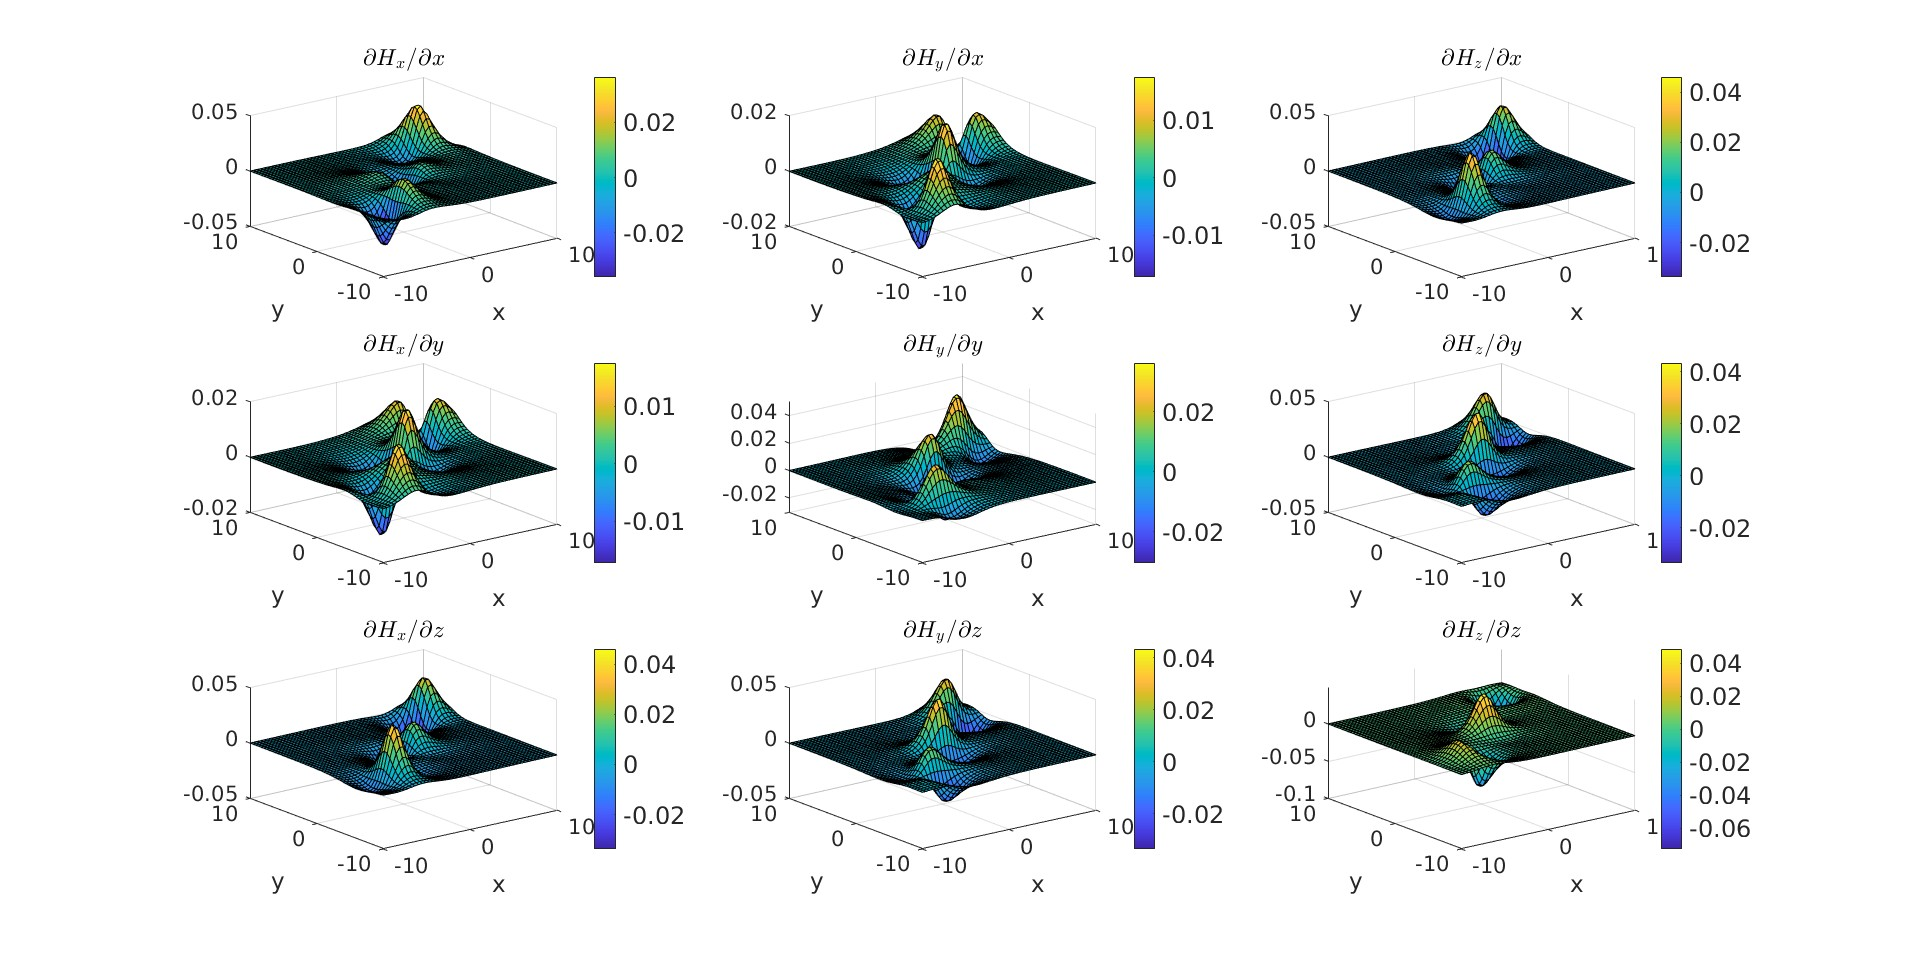
\includegraphics[width=1.4\textwidth]{images/gradients_rotated_multi_num.jpg}
\caption{Plot of the gradient tensor ${}^r \mathbf{G}_{\text{tot}}$ elements
when computed numerically in the case of multiple sources positioned at  $(0,0,0)$, $(-6,-6,0)$, and $(7,7,0)$;
with rotations $\mathbf{R}^t_r$ and $\mathbf{R}_t^g$.}
\label{fig:gradients_rotated_multi_num}
\end{figure}

%NSS NUMERICAL ROTATIONS 
\begin{figure}
\centering
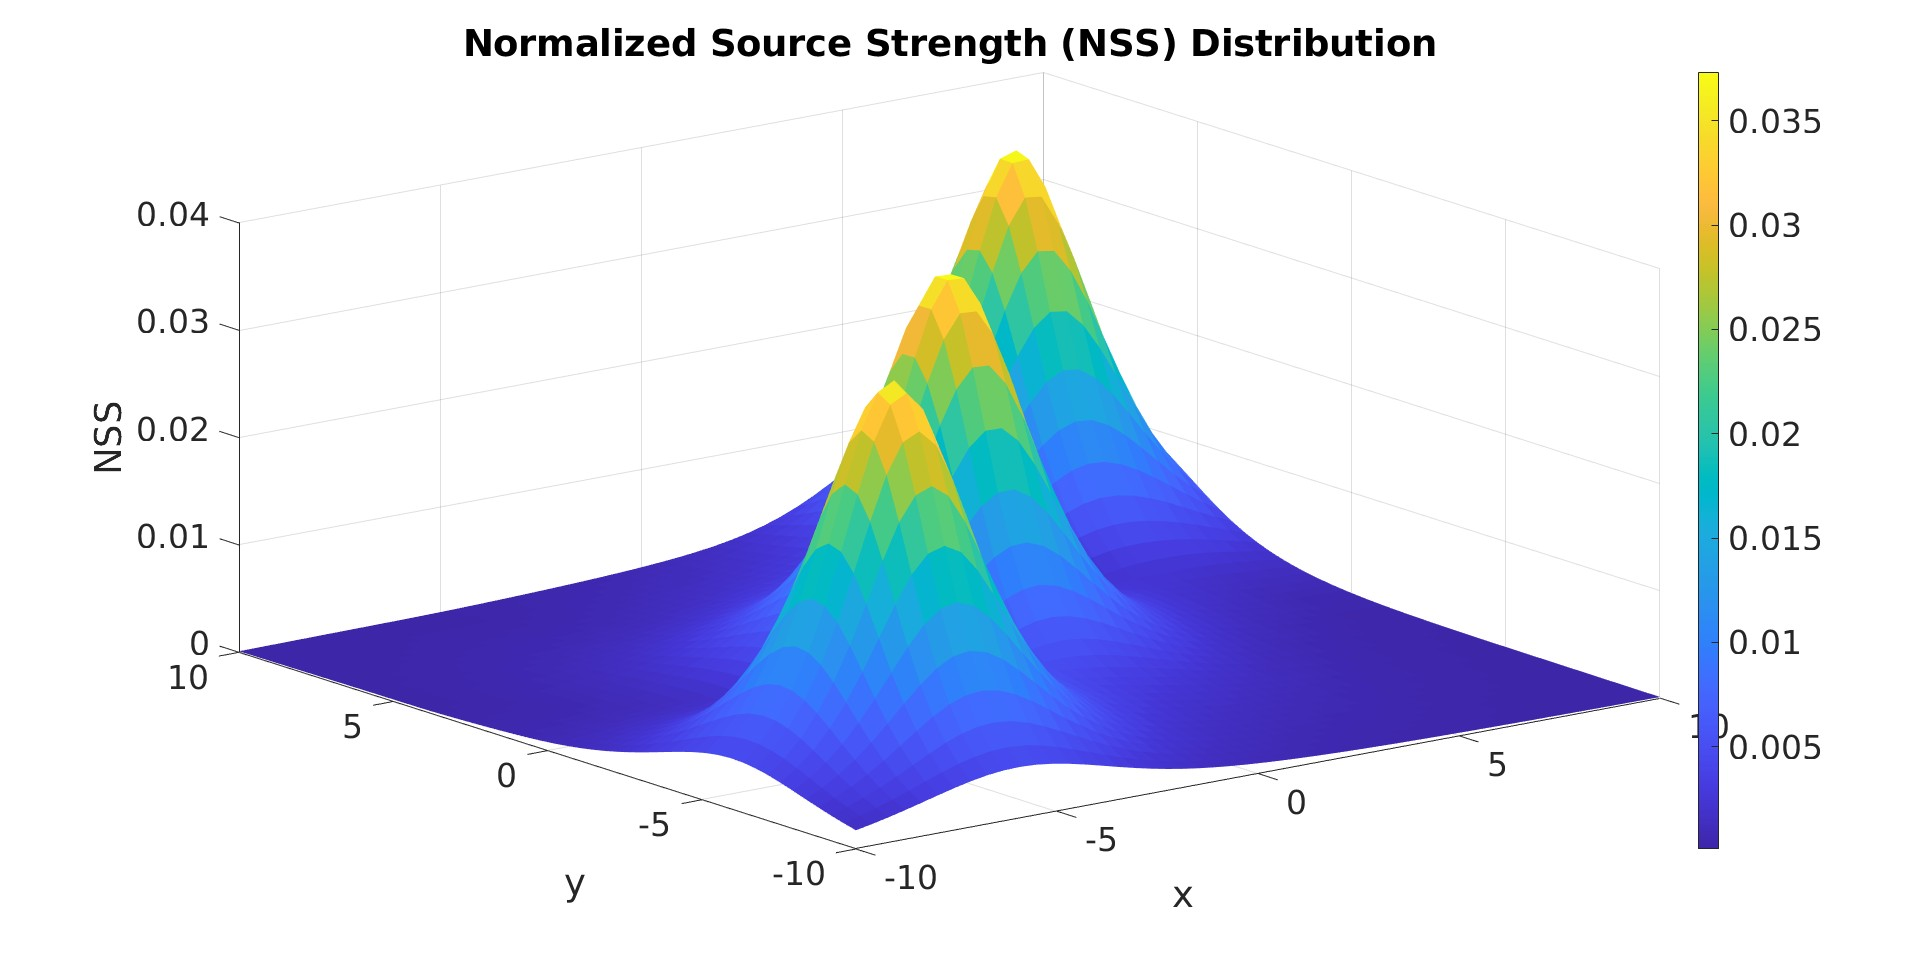
\includegraphics[width=0.8\textwidth]{images/NSS_rotated_multi_num.jpg}
\caption{Plot of the NSS computed numerically in the case of multiple sources positioned at  $(0,0,0)$, $(-6,-6,0)$, and $(7,7,0)$;
with rotations $\mathbf{R}^t_r$ and $\mathbf{R}_t^g$.}
\label{fig:NSS_rotated_multi_num}
\end{figure} 

By looking at Fig.\ref{fig:gradients_multi_num} and Fig.\ref{fig:gradients_rotated_multi_num}
we can observe again that the gradients vary in the case in which the reference
frames $F_{t_i}$, $F_r$ and $F_g$ have different orientations with respect to one another;
however the matrix mantains the symmetry property.
Instead, by comparing Fig.\ref{fig:NSS_multi_num} with Fig.\ref{fig:NSS_rotated_multi_num}
we verify that the NSS distribution is rotationally invariant, like in all the other cases both with 
single or multiple victims.


\subsection{Final Model}
In the final model of the multiple-victims scenario, we consider an ARTVA transmitter attached 
to each $i$-th victim among the $n \in \mathbb{N}$ victims, where \( i = 1, \ldots, n \).
In addition, we employ a swarm of $m \in \mathbb{N}$ UAVs to locate the position
of at least $m$ victims if $m \min n$, otherwise to localize them all.
We assume the position of the $j$-th drone, \( \mathbf{p}_{r_j}(\tau_k) \in \mathbb{R}^3 \) ,
to be known at every sample time \( \tau_k \), where \( k, j \in \mathbb{N} \) 
and \( j = 1, \ldots, m \).
We also consider each UAV to be equipped, with an ARTVA receiver, or any other 
instrument capable of detecting the electromagnetic field at different points,
like the TAMs in \cite{NSS_single_localization}.
Since ARTVAs are the most commonly used instruments we compute the NSS using the
analytical method, but we note that the numerical method could be employed
in the precence of any other suitable equipment.

Knowing the position of the $j$-th drone $\mathbf{p}_{r}(\tau_k)$, 
we compute the NSS using the analytical expression of the gradient tensor, which depends
only on the position of the receiver drone in the transmitter frame
${}^{t_i} \mathbf{p}(\tau_k)$.
From Eq. \ref{eq:pt_multi} we express the position of each $j$-th drone
in the relative trasmitter frame $F_{t_i}$ of each $i$-th source:
\begin{equation}
    {}^{t_i} \mathbf{p}(\tau_k) = {R^g_{t_i}}^\top \, \left( \mathbf{p}_{r}(\tau_k) - \mathbf{p}_{t_i}(\tau_k) \right)
\end{equation}
Then, we compute the gradient tensor matrix relative to a single source 
${}^{t_i} \mathbf{G}_i({}^{t_i} \mathbf{p})$ using the analytical expression in \ref{eq:G_analit}:
\begin{equation}
    {}^{t_i} \mathbf{G}_i = \frac{1}{r_i^{5/2}}
    \scalebox{0.90}{$
    \begin{bmatrix}
    3 x_i (-2 x_i^2 + 3y_i^2 + 3z_i^2) & 3 y_i (-4 x_i^2 + y_i^2 + z_i^2) & 3 z_i (-4x_i^2 + y_i^2 + z_i^2) \\
    3 y_i (-4 x_i^2 + y_i^2 + z_i^2) & 3 x_i (x_i^2 - 4 y_i^2 + z_i^2) & -15 x_i y_i z_i \\
    3 z_i (-4 x_i^2 + y_i^2 + z_i^2) & -15 x_i y_i z_i & 3 x_i (x_i^2 + y_i^2 - 4 z_i^2)
    \end{bmatrix}
    $}
\end{equation}
where $r_i$ is the distance between the $i$-th source and the receiver position 
$\mathbf{p}_{r}(\tau_k)$ and  $(x_i, y_i, z_i)$ are the coordinates 
relative to ${}^{t_i} \mathbf{p}(\tau_k)$.

\noindent
\\
Subsequently, we sum all the gradient tensors rotated in the common receiver frame $F_{r}$
to obtain ${}^{r} \mathbf{G}_{\text{tot}} ({}^{t_1} \mathbf{p}, \dots {}^{t_n} \mathbf{p})$, in the same way as Eq. \ref{eq:G_tot}.

Finally, we conpute the eigenvalues of total gradient 
tensor to find the NSS relative to all sources using Eq.\ref{eq:NSS},
 at each time step \( \tau_k \):
\begin{equation}
    \text{NSS}_\text{tot}(\tau_k) = \sqrt{{\lambda_{\text{tot}_2}}^2 - \lambda_{\text{tot}_1} \lambda_{\text{tot}_3}}
    \label{eq:NSS_multi_final}
\end{equation}
where $\lambda_{\text{tot}_1}$, $\lambda_{\text{tot}_2}$ and $\lambda_{\text{tot}_3}$
are the ordered (from min to max) eigenvalues relative to the total magnetic gradient tensor.

\noindent
\\
Therefore, we model the intensity of the signal received by each UAV using the NSS
as an output funcion of the form \( y_j : \mathbb{R}^3 
\times \mathbb{R} \rightarrow \mathbb{R} \):
\begin{equation}
y_j(\mathbf{p}_{r}, \mathbf{p}_{t_i}, \tau_k) = \mathbf{\Phi}(\mathbf{p}_{r}, \mathbf{p}_{t_i}, \tau_k) + 
w_t(\mathbf{p}_{r}, \mathbf{p}_{t_i}, \tau_k)
\label{eq:received_signal}
\end{equation}
where $\mathbf{\Phi}(\mathbf{p}_{r}, \mathbf{p}_{t_i}, \tau_k)$ is the NSS
relative to each $j$-th receiver and 
and \( w : \mathbb{R}^3 \times \mathbb{R} \rightarrow \mathbb{R} \) 
represents the measurement noise related to the electromagnetic interference,
defined in \ref{eq:H_rotated_noise}.

\subsection{MY ALGORITHM NAME}
In this work, we present MY ALGORITHM NAME, a modification of the PSO
which....

\subsubsection{Particle Swarm Oprimization}
The PSO algorithm is an intelligent population-based stochastic optimization technique 
that simulates the behavior of a natural biological swarm. 
As already mentioned, each “particle” represents a potential solution in the search space
and it updates its velocity and position based on the historical best positions 
of both the individual and the entire population.
 
\noindent
\\
We asssume that $m$ seeker drones act as $m$ particles moving in the search-space, 
like in \cite{3}; therefore we denote the position of each particle as the $j$-th UAV
$\mathbf{p}_{r_j}(\tau_k) \in \mathbb{R}^2$, at the $\tau_k$ iteration.
\noindent
\\
\textbf{Assumption}
\\
We make the assumption that the UAVs fly at a constant height; therefore we can
simplify the control task on the 2D plane.
Furthermore, in the standard PSO algorithm \cite{PSO_original}, the particles are randomly 
initialized within the search-space. In contrast, our model assumes that the UAVs 
start from the center of the space.

The value of the function to be optimized, usually
called the cost function, is evaluated at the position of the particle at 
each time step $\tau_k$ and it is modeled using the signal 
received by the receiver UAVs at its current location
\( y_j : \mathbb{R}^2 
\times \mathbb{R} \rightarrow \mathbb{R} \), expressed in 
Eq.\ref{eq:received_signal}.

The multiple-source seeking task is performed on a search-space $\Omega$ 
where the multiple victims are located, 
defined as the solution space where the $y_j$ funtion is maximized.
\[
\Omega = (x, y, z) \, \text{s.t.} \,
\begin{cases}
    X_{\min} \leq x \leq X_{\max}, \\
    Y_{\min} \leq y \leq Y_{\max}, \\
    Z_{\min} \leq z \leq Z_{\max}
\end{cases}
\]
where $X_{\min}$, $X_{\max}$, $Y_{\min}$, and $Y_{\min}$ denote the horizontal
boundaries. and $Z_{\min}$ and $Z_{\max}$ denote the ground level and
the highest limit.
\noindent
\\
\textbf{Assumption}
\\
We limit the search-space to the 2D plane as well, as we are not interested
in determining the burial depth of the victims, 
which would need the emplyment of different a
invariant from the NSS.
Instead, we fix the $z$ coordinate to the ground level for all the victims;
while we assume a constant flying height of 3m for the UAVs, as already mentioned.

\noindent
\\
The standard PSO algorithm iterative update of each particle's velocity
(Eq.~\ref{eq:model_velocity}) and position (Eq.~\ref{eq:model_position})
in the search-space to improve its solution:
\begin{align}
    \mathbf{v}_{j}(\tau_k+1) &= \omega \mathbf{v}_{j}(\tau_k) 
    + c_1 r_1 \big(\mathbf{pbest}_{j}(\tau_k) - \mathbf{p}_{r_j}(\tau_k)\big) + \notag \\
    &\quad + c_2 r_2 \big(\mathbf{gbest}(\tau_k) - \mathbf{p}_{j}(\tau_k)\big) \label{eq:model_velocity} \\
    \mathbf{p}_{r_j}(\tau_k + 1) &= \mathbf{p}_{r_j}(\tau_k) + \mathbf{v}_{j}(\tau_k+1) \label{eq:model_position}
\end{align}
where $\mathbf{pbest}_j$ represents the $j$-th particle's individual best position vector  
, $\mathbf{gbest}$ the global best position vector, $\omega$ is the inertia weight,
$c_1$ and $c_2$ are positive constants, and $r_1, r_2 \sim \textit{U}(0,1)$ are random variables 
uniformly distributed over the interval $[0, 1]$.

A best previous position is where a particle obtains the 
maximum value of the output function in its search
history.
In \ref{eq:model_velocity}, velocity $\mathbf{v}_{j}(\tau_k+1)$ 
consists of three terms: the effect of drone’s previous velocity, 
effect of its best known position and effect of global best
known position.
While the inertia weight is critical in balancing global and local search. 
A larger inertia weight facilitates global exploration while a smaller one
facilitates local exploitation.

In the standard PSO algorithm, there is only one global best particle, 
which means that only one optimal solution can be found. This limitation 
poses a challenge when dealing with our problem, where we are looking for multiple sources, 
and therefore, multiple local and global optima exist. To address this challenge, 
we employ the same strategy of the modified version of the PSO algorithm \cite{PSO_IMPORTANT}. 
In this modification, the swarm is divided into $M$ subpopulations, each tasked with exploring 
different regions of the search space. Following this idea, the \textit{gbest} is referred to as 
the best particle of each subpopulation, not as the global best particle in the whole population. 
This means that these $M$ best particles are separately able to catch different optima, 
at most $M$ optima.

\noindent
\\
In addition, we perform further modifications to the PSO algorithm,
we introduce physical constraints as already done in \cite{3} and 
an exclusion zone mechanism.

Firstly, the UAVs are confined to the 
search-space and secondly their velocity is 
capped to a max value to avoid speed "explosion", \cite{3}.

The constraints are formulated as follows:
\[
\begin{cases}
    \mathbf{p}_{r_j}(\tau_k + 1) = \mathbf{p}_\text{lim}, & \text{if } \mathbf{p}_{r_j}(\tau_k) \notin \Omega, \\
    \mathbf{v}_j(\tau_k + 1) = v_{\text{max}} \frac{\mathbf{v}_j(\tau_k)}{\|\mathbf{v}_j(\tau_k)\|}, & \text{if } \|\mathbf{v}_j(\tau_k)\| > v_{\text{max}}.
\end{cases}
\]
where \( \mathbf{p}_\text{lim} \) is the nearest point on the boundaries of the search space \( \Omega \), 
and \( v_{\text{max}} \) denotes the maximum allowed step length.

\noindent
This means that:
\begin{itemize}
    \item If the UAV exits the search space limits (i.e., \( \mathbf{p}_{r_j}(\tau_k+1) \notin \Omega \)), 
    its position is corrected to the nearest boundary point of \( \Omega \) 
    in the next iteration.
    \item If the magnitude of the velocity \( \|\mathbf{v}_j(\tau_k + 1)\| \) 
    exceeds the maximum allowable speed \( v_{\text{max}} \), 
    then the velocity is scaled down to \( v_{\text{max}} \), 
    while maintaining the same direction.
\end{itemize}

\subsection{Exclusion Zone Mechanism}
In order to avoid clustering around the same source 
and to ensure that the swarm does not converge only 
on a few sources, we introduce an exclusion zone mechanism. 
This strategy enforces additional positional constraints 
on the drones by leveraging the fact that each drone 
knows its current position in the search space.

\noindent
\\
A drone \( j \) defines an exclusion zone when it detects a source 
with a signal strength, the NSS, greater than a predefined threshold 
\( \text{NSS}_{\text{thresh}} \). The exclusion zone is represented 
as a circular region, centered around the position of the drone, defined by:
\[
\mathcal{E}_j = \{ \mathbf{p} \in \mathbb{R}^3 \mid \|\mathbf{p} - \mathbf{c}_j\| 
\leq r_{\text{excl}} \},
\]
where:
\begin{itemize}
    \item \( \mathbf{c}_j \) is the center of the exclusion zone, 
    corresponding to the position of the drone when the source 
    is detected (\( \mathbf{p}_{r_j}(\tau_k) \)).
    \item \( r_{\text{excl}} \) is the radius of the exclusion zone, 
    chosen experimentally.
\end{itemize}

\noindent
\\
Instead, a drone \( j \) shares the center \( \mathbf{c}_j \) and radius 
\( r_{\text{excl}} \) of its exclusion zone with neighboring drones 
if they are within the communication range \( r_{\text{comm}} \). 
A neighboring UAV \( l \) receives the exclusion zone when:
\[
\|\mathbf{p}_{r_l}(\tau_k) - \mathbf{p}_{r_j}(\tau_k)\| \leq r_{\text{comm}}.
\]
Each drone maintains a list of shared exclusion zones 
\( \mathcal{E}_\text{shared} \), which is defined as:
\[
\mathcal{E}_\text{shared} = \{\mathcal{E}_1, \mathcal{E}_2, \dots, \mathcal{E}_k\}
\]
which is an unordered and incomplete set of 
where the union is over all exclusion zones shared by neighboring drones.

\paragraph{Checking}
Each drone continuously checks whether its current position 
\( \mathbf{p}_{r_j}(\tau_k) \) lies within any shared exclusion zone. 
This is verified by:
\[
\mathbf{p}_{r_j}(\tau_k) \in \mathcal{E}_\text{shared}.
\]

\paragraph{Avoidance}
If a drone \( j \) finds itself within a shared exclusion zone at time \( \tau_k \), 
it computes a new goal position \( \mathbf{p}_{r_j}^{\text{goal}}(\tau_k + 1) \) 
to escape the zone. The avoidance mechanism follows these steps:

\[
\mathbf{d}_j(\tau_k) = \mathbf{c}_j(\tau_k) - \mathbf{p}_{r_j}(\tau_k),
\]
where \( \mathbf{d}_j(\tau_k) \) is the direction vector pointing away 
from the exclusion zone center \( \mathbf{c}_j(\tau_k) \), and 
\( \mathbf{p}_{r_j}(\tau_k) \in \mathcal{E}_j(\tau_k) \).

The goal position for the drone in the next iteration is then calculated as:
\[
\mathbf{p}_{r_j}^{\text{goal}}(\tau_k + 1) = \mathbf{p}_{r_j}(\tau_k) 
+ \alpha \frac{\mathbf{d}_j(\tau_k)}{\|\mathbf{d}_j(\tau_k)\|},
\]
where:
\begin{itemize}
    \item \( \alpha \): Step size parameter that determines 
    the distance the drone moves away from the exclusion zone.
    \item \( \mathbf{p}_{r_j}^{\text{goal}}(\tau_k + 1) \): The computed 
    goal position outside the exclusion zone.
    \item \( \|\mathbf{d}_j(\tau_k)\| \): Norm (magnitude) of the direction 
    vector \( \mathbf{d}_j(\tau_k) \), which is used for normalization.
\end{itemize}

Once the drone reaches \( \mathbf{p}_{r_j}^{\text{goal}}(\tau_k + 1) \), 
it resumes the PSO algorithm, continuing to search for new sources. 
This mechanism ensures the drone moves directly away from the 
exclusion zone while covering a distance proportional to \( \alpha \).


\subsubsection{Communication Topology}

\subsubsection{Metrics}
--- we terminate when the value is greater than a threshold

in \cite{3}
qui si parla di standard PSO chiamato SPSO
The swarm size is determined by , where is the
dimension of the search space. Standard value of the parameters
are as follows:


To evaluate the seeking time and energy consumption, we define
. Thus, provides a measure on
the total “time” to complete a search since it is proportional to
search time based on the assumption that all seekers have equal
speed. The actual time cannot be computed in simulations due to
the lack of the concept of speed, but serves the same
purpose.
In addition, we also count the number of iterations ,
measure the total distance traveled by all robots 


\section{UAV Dynamics}
Each Uav folows this dynamics
Assuming the receiver frame coincides with the body frame, as in \cite{similar-main}, 
the UAV is modeled as a quadrotor. Its dynamics are described using Newton's 
second law for both translational and rotational motion. The motion is expressed 
in terms of the inertial frame \( F_i \) and the body frame \( F_b \).

---

\subsection{Translational Dynamics}

The position of the UAV's center of gravity is represented by \( \mathbf{p} \in \mathbb{R}^3 \), 
expressed in the inertial frame \( F_i \). Its derivative, \( \dot{\mathbf{p}} \), denotes the linear velocity.

Using Newton's second law, the translational dynamics are:
\[
M \frac{\mathrm{d}^2 \mathbf{p}}{\mathrm{d} t^2} = \mathbf{F}_{\text{tot}},
\]
where:
\begin{itemize}
    \item \( M \): UAV mass.
    \item \( \mathbf{F}_{\text{total}} \): Total force acting on the UAV.
\end{itemize}

The total force in the inertial frame \( F_i \) includes:
\begin{itemize}
    \item \textbf{Thrust Force \( \mathbf{f}_\text{thrust} \):}
    \[
    \mathbf{f}_\text{thrust} = -u_f \mathbf{R}_b^i \mathbf{e}_3,
    \]
    where:
    \begin{itemize}
        \item \( u_f \geq 0 \): Control force aligned with the body \( z \)-axis.
        \item \( \mathbf{e}_3 = [0, 0, 1]^\top \): Unit vector along the \( z \)-axis.
        \item \( \mathbf{R}_b^i \in \text{SO}(3) \): Rotation matrix mapping vectors from \( F_b \) to \( F_i \).
    \end{itemize}
    \item \textbf{Gravitational Force \( \mathbf{f}_g \):}
    \[
    \mathbf{f}_g = M g \mathbf{e}_3,
    \]
    where \( g \) is the gravitational constant.
    \item \textbf{Disturbance Forces \( \mathbf{d}_f \):}
    \[
    \mathbf{d}_f = \begin{bmatrix} d_{f,x} \\ d_{f,y} \\ d_{f,z} \end{bmatrix},
    \]
    representing external forces such as wind and drag.
\end{itemize}

The translational dynamics in the inertial frame are:
\[
M \ddot{\mathbf{p}} = -u_f \mathbf{R}_b^i \mathbf{e}_3 + M g \mathbf{e}_3 + \mathbf{d}_f.
\]

---

\subsubsection{Rotational Dynamics}

The angular velocity \( \boldsymbol{\omega} \in \mathbb{R}^3 \) is expressed in the body frame \( F_b \). 
Newton's second law for rotational motion gives:
\[
\mathbf{J} \dot{\boldsymbol{\omega}} = \boldsymbol{\tau} - \boldsymbol{\omega} \times (\mathbf{J} \boldsymbol{\omega}),
\]
where:
\begin{itemize}
    \item \( \mathbf{J} \in \mathbb{R}^{3 \times 3} \): Inertia matrix of the UAV, symmetric and positive definite (\( \mathbf{J} = \mathbf{J}^\top > 0 \)).
    \item \( \boldsymbol{\tau} \in \mathbb{R}^3 \): Control torque vector.
    \item \( \boldsymbol{\omega} \times (\mathbf{J} \boldsymbol{\omega}) \): Coriolis torque.
\end{itemize}

The rotation matrix \( \mathbf{R}_b^i \in \text{SO}(3) \) evolves as:
\[
\dot{\mathbf{R}}_b^i = \mathbf{R}_b^i \mathbf{S}(\boldsymbol{\omega}),
\]
where \( \mathbf{S}(\boldsymbol{\omega}) \) is the skew-symmetric matrix:
\[
\mathbf{S}(\boldsymbol{\omega}) = 
\begin{bmatrix} 
0 & -\omega_z & \omega_y \\ 
\omega_z & 0 & -\omega_x \\ 
-\omega_y & \omega_x & 0 
\end{bmatrix}.
\]

---

\subsubsection{Full Dynamics in the Inertial Frame}

Combining translational and rotational dynamics, the UAV's motion in the inertial frame \( F_i \) is:
\[
M \ddot{\mathbf{p}} = \mathbf{R}_b^i \begin{bmatrix} 0 \\ 0 \\ -u_f \end{bmatrix} + M g \mathbf{e}_3 + \mathbf{d}_f,
\]
\[
\mathbf{J} \dot{\boldsymbol{\omega}} = \boldsymbol{\tau} - \boldsymbol{\omega} \times (\mathbf{J} \boldsymbol{\omega}),
\]
where the inputs \( u_f \) (thrust) and \( \boldsymbol{\tau} \) (torques) are used for control purposes.

The orientation matrix \( \mathbf{R}_b^i \) evolves as:
\[
\dot{\mathbf{R}}_b^i = \mathbf{R}_b^i \mathbf{S}(\boldsymbol{\omega}).
\]

---

\subsubsection{Additional Notes on Rotation Matrices}

The rotation matrix \( \mathbf{R}(t) \) satisfies the orthogonality condition:
\[
\mathbf{R}(t) \mathbf{R}^\top(t) = \mathbf{I}.
\]
Its time derivative \( \dot{\mathbf{R}}(t) \) obeys:
\[
\dot{\mathbf{R}}(t) \mathbf{R}^\top(t) + \mathbf{R}(t) \dot{\mathbf{R}}^\top(t) = 0.
\]

This ensures that the skew-symmetric matrix \( \mathbf{S}(\boldsymbol{\omega}) \) represents angular velocity in the body frame:
\[
\mathbf{S}(\boldsymbol{\omega}) \mathbf{R}(t) = \dot{\mathbf{R}}(t).
\]


\section{Control}
the purpose of this work is not to control the attitude (orientation), 
but the position and velocity
